\documentclass{article}

\usepackage[utf8]{inputenc}
\usepackage[dvipsnames]{xcolor}
\usepackage{lmodern}
\usepackage{graphicx}
\usepackage{tabularx}
\graphicspath{ {./images/} }
\usepackage{imakeidx}
\makeindex[columns=3, title=Alphabetical Index, intoc]

\usepackage{tabularx}
\usepackage{amsmath}
\usepackage{paralist}
\usepackage{enumitem}
\usepackage{hyperref} %\usepackage[hidelinks]{hyperref} %per togliere bordi rossi
\usepackage{makecell}
\usepackage{caption}
\usepackage[maxfloats=256]{morefloats}
\maxdeadcycles=1000

\usepackage[official]{eurosym}
\DeclareUnicodeCharacter{20AC}{\euro{}}

\newcounter{ucCounter}
\stepcounter{ucCounter}
\newcommand{\lastUC}{\theucCounter}
\newcommand{\nextUC}{\stepcounter{ucCounter}{\theucCounter}}

\author{Agosta, Belli, Emili, Giacchini, Luciani}

\begin{document}

\begin{center}
    \sffamily{\fontsize{50}{48} \selectfont \textcolor{red}{Nexi}\textcolor{green}{Fy}}
\end{center}

\begin{center}
    \itshape{\fontsize{20}{48} \selectfont streaming to your pocket}
\end{center}

\bigskip\bigskip\bigskip

\begin{flushleft}
    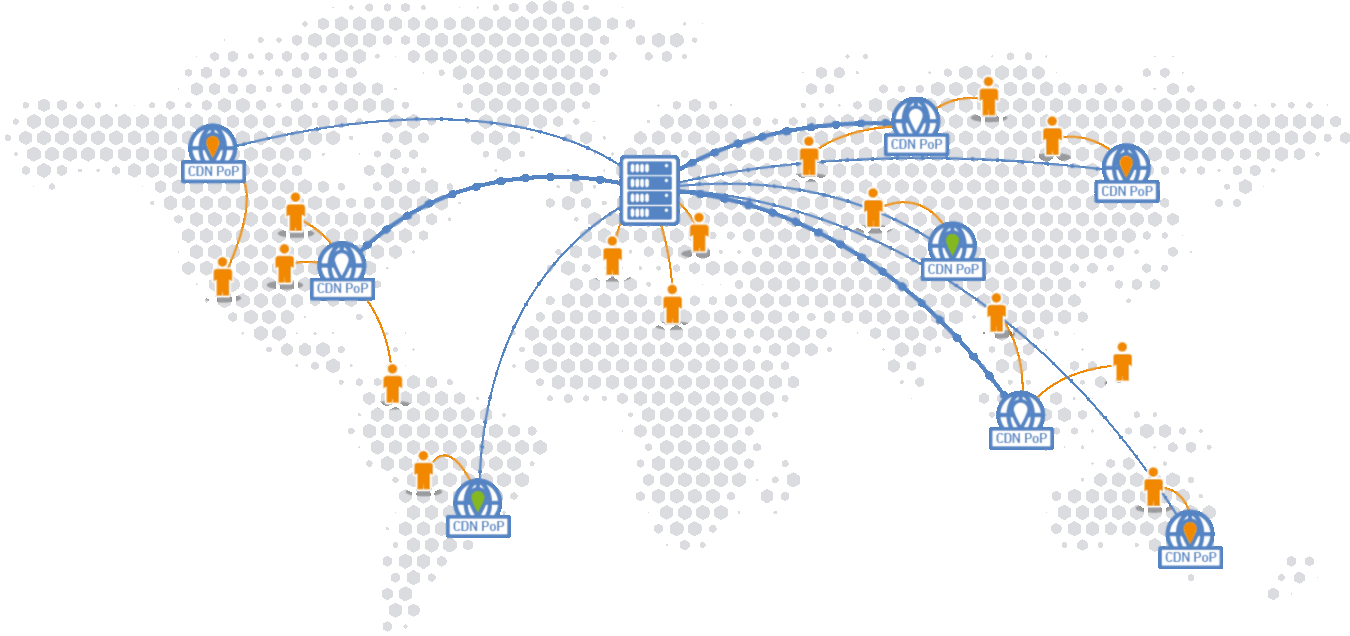
\includegraphics[scale=1]{images/worldCDN.png}
\end{flushleft}

\newpage
\printindex

\tableofcontents

\newpage
\section{\itshape{Glossario}}
 In questa sezione saranno esplicitati tutti i termini necessari alla comprensione del progetto.

\begin{itemize}
	%\item  \textbf{multimedia-manager}: servizio usato da partner per la gestione (caricamento/eliminazione) dei propri video e/o tracce audio. %viene citato solamente qui nel glossario
	\item \textbf{Piano di abbonamento}: pacchetto di funzionalità, acquistabile dagli utenti per un certo periodo (e rinnovabile alla fine del periodo). A volte è indicato impropriamente come "abbonamento"
	\item \textbf{API}: interfaccia offerta all'esterno di un sistema, per poter usare delle funzionalità interne al sistema
	\item \textbf{CDN}: sistema di server largamente distribuita, usata per la distribuzione di contenuti quali tracce video e audio.
	\item \textbf{ORM}: tecnica per interfacciarsi con basi di dati relazionali, astraendo dall'implementazione del dbms
	\item \textbf{Piattaforma}: componente del sistema accessibile dagli utenti.
	\item \textbf{Server}: macchina logica (composta da uno o piu macchine fisiche) su cui risiede la piattaforma in parte o nella sua totalità.
	\item \textbf{RUP}: Rational Unified Process, processo di sviluppo basato su fasi temporali, iterazioni e attività.
	\item \textbf{Risorsa Multimediale}: intendiamo un file di tipo multimediale, quindi un video, una canzone, ecc. (a volte è indicata solamente come risorsa)
	\item \textbf{Prodotto}: si intende un singolo prodotto video o audio creato da un partner (e.g: un singolo film, una singola canzone, un singolo episodio di una serie tv, ecc.)
	\item \textbf{Playlist}: lista ordinata di prodotti
	\item \textbf{Contenuto}: un singolo prodotto o una playlist
\end{itemize}
\index{Index}

\newpage
\section{\itshape{Visione del Sistema}}
\textbf{NexiFy} è una piattaforma di streaming multimediale on demand che offre contenuti quali film, serie tv, brani e video musicali e altre forme di intrattenimento. Il servizio è fruibile sia via web che da app mobile.\\

La fruizione dei contenuti avviene attraverso un singolo player audio / video:
\begin{itemize}\item per la riproduzione di film o serie tv entrambe le tracce video e audio vengono riprodotte in contemporanea. L’utente può scegliere la qualità di riproduzione, manualmente o automaticamente, in base alle sue preferenze e disponibilità di connessione a internet. Possono essere mostrati anche dei sottotitoli (se disponibili).
    \item per la riproduzione di musica ci sono due scenari diversi (in entrambi i casi il brano può essere ascoltato con l’app in background, inibendo quindi la traccia video) :
    \begin{enumerate}
        \item il brano è accompagnato dal relativo video musicale; in questo caso vengono riprodotte entrambe le tracce audio e video contemporaneamente.
        \item il brano non è accompagnato dal video musicale; in questo caso viene riprodotta la sola traccia audio e al posto della traccia video, viene mostrata la copertina dell’album relativo al brano oppure i lyrics del brano in tempo reale (in base alla scelta dell’utente e alla disponibilità dei lyrics).
    \end{enumerate}
\end{itemize}
    
Gli utenti della piattaforma si dividono in due categorie: partner e iscritti.\\

I contenuti sono caricati da partner che sottoscrivono un contratto di collaborazione, pagando una quota annuale uguale per tutti ma modificabile nel corso del tempo. Questi ultimi ricevono un compenso in base al numero di riproduzioni che hanno ottenuto sui loro contenuti.\\

Gli iscritti sono coloro che usufruiscono del servizio; essi hanno la possibilità di scegliere diversi profili di abbonamento definibili a piacere tramite apposite funzioni di creazione a associazione degli abbonamenti alle varie funzionalità offerte dal sistema.\\

Questo servizio dà la possibilità agli iscritti interessati di visualizzare film e serie tv e ascoltare brani musicali sottoscrivendo un singolo abbonamento. Questo porta ad essi un risparmio di denaro, in quanto non è necessario iscriversi a diversi servizi il cui costo totale ammonterebbe ad una quota mensile maggiore.\\

\subsection{\itshape{Vincoli}}
NexiFy si riserva la possibilità di rimuovere qualsiasi contenuto video e/o audio presente sulla piattaforma che, dopo previa verifica, non rispetta la linee guida dei TOS.
In particolare è vietato il caricamento di qualsiasi traccia audio/video con contenuti sessualmente espliciti o che promuovono o giustificano l'uso della violenza contro persone o gruppi in base a razza, etnia, religione, disabilità fisiche, sesso, età, nazionalità né contenuti il cui scopo sia l'incitamento all'odio sulla base di tali caratteristiche.

\index{Index}

\subsection{\itshape{Configurazione del Sistema alla Consegna}}
Alla consegna del sistema prevediamo, già inclusi in esso, i seguenti abbonamenti designati e pensati per gli utenti:
\begin{itemize}
    \item Free (0 € / mese ) che darà accesso alle seguenti funzioni: 
	\begin{itemize}
   		\item Ascoltare brani musicali presenti sulla piattaforma \textbf{con} limiti di scelta di riproduzione e intermezzi pubblicitari;
		\item Visionare episodi pilota di serie tv;
		\item Visionare trailer di film.
	\end{itemize}
    \item Music (9.99 € / mese) che darà accesso alle seguenti funzioni:
	\begin{itemize}
   		\item Ascoltare brani musicali presenti sulla piattaforma \textbf{senza} limiti di scelta di riproduzione e intermezzi pubblicitari;
		\item Scaricare su dispositivo, tramite app mobile, brani musicali per usufruirne offline;
		\item Visionare episodi pilota di serie tv;
		\item Visionare trailer di film.
	\end{itemize}
    \item Premium (14.99 € / mese) che darà accesso alle seguenti funzioni:
	\begin{itemize}
   		\item Ascoltare brani musicali presenti sulla piattaforma \textbf{senza} limiti di scelta di riproduzione e intermezzi pubblicitari;
		\item Scaricare su dispositivo, tramite app mobile, brani musicali per usufruirne offline;
		\item Visionare tutti gli episodi delle serie tv presenti sulla piattaforma;
		\item Scaricare su dispositivo, tramite app mobile, episodi di serie tv per usufruirne offline;
		\item Visionare tutti i film presenti sulla piattaforma.
		\item Scaricare su dispositivo, tramite app mobile, film per usufruirne offline;
	\end{itemize}
	
	\item Partner (300 € / anno) che darà accesso alle seguenti funzioni:
	\begin{itemize}
   		\item Pubblicazione di video
		\item Pubblicazione di brani musicali
		\item Modifica/rimozione di video
		\item Modifica/rimozione di brani musicali
		\item Ricevere pagamenti in base alle visualizzazioni sui propri contenuti
	\end{itemize}
\end{itemize}


La CDN fornita coprirà l’intera area geografica globale arrivando in tempi ragionevoli a tutti gli utenti. Inoltre supporterà un numero massimo di XXXX utenti.


\index{Index}

\subsection{\itshape{Vincoli}}
\begin{itemize}
\item NexiFy si riserva di modificare la quota annuale per i partner.
\item NexiFy si riserva di rimuovere ogni contenuto considerato non idoneo ad essere visualizzato o riprodotto dagli utenti.
\item In caso di contenuti particolari, prima della riproduzione l'utente verrà informato, dando la possibilità di evitare contenuti non desiderati.
\item In particolare è vietato il caricamento di qualsiasi traccia audio/video con contenuti sessualmente espliciti o che promuovono o giustificano l'uso della violenza contro persone o gruppi in base a razza, etnia, religione, disabilità fisiche, sesso, età, nazionalità né contenuti il cui scopo sia l'incitamento all'odio sulla base di tali caratteristiche. 
\item NexiFy può creare/modificare/rimuovere profili di abbonamento. 
\item Qualsiasi risorsa audio o video scaricata tramite l'app mobile sarà codificata in modo tale da rendere il file accessibile \textbf{solo ed esclusivamente} tramite il player dell'app stessa onde evitare una riproduzione non consentita di questi.
\end{itemize}
 


\index{Index}

\newpage
\section{\itshape{Studio di Fattibilità}}
\subsection{Aspetto tecnologico}
Per la realizzazione del sistema sarà necessario l'utilizzo di CDN, in modo da distribuire i contenuti multimediali in maniera efficiente e mantenendoli sempre accessibili per gli utenti. Deve inoltre essere possibile, in maniera efficiente, estrarre dati e statistiche dalla CDN (come per esempio quante volte è stato richiesto un certo video in una certa zona). Saranno necessarie basi di dati relazionali cloud-based per mantenere informazioni su dati utenti (oltre alle informazioni di base, anche le eventuali playlist musicali create, ecc), e implementando funzionalità lato server per gestire le richieste degli utenti, la loro autenticazione e altro. Verrà inoltre utilizzato un ORM per garantire semplicità di migrazione ad un'altra tecnologia di memorizzazione dati permettendo di rendere indipendente il codice dalla base di dati.\\
La fattibilità del progetto dal punto di vista tecnologico segue dalla grande disponibilità di aziende che offrono servizi cloud, tra cui CDN: per esempio AWS CloudFront. Questi servizi includono anche delle API per interfacciarsi in maniera efficiente con la CDN. Notiamo che questi servizi vengono già usati da piattaforme simili a NexiFy, e che sono risultate in grado di scalare a livello mondiale (ad esempio Prime Video usa AWS CloudFront). Anche per quanto riguarda i database esistono numerose soluzioni cloud affidabili.
%Il mantenimento dei dati riguardanti gli utenti sarà conforme alle politiche GDPR per garantire la privacy secondo le leggi europee.\\


%Per la realizzazione della piattaforma sarà necessario l’utilizzo di CDN per distribuire sul territorio contenuti multimediali mantenendo questi ultimi sempre accessibili in maniera ottimale da qualsiasi posizione geografica. Deve inoltre essere possibile, in maniera efficiente, estrarre dati e statistiche sugli accessi alla CDN. Si useranno basi di dati relazionali cloud-based per mantenere informazioni su dati utenti, e implementando funzionalità lato server per gestire le richieste degli utenti, la loro autenticazione e altro.Verrà inoltre utilizzato un ORM per garantire semplicità di migrazione ad un'altra tecnologia di memorizzazione dati permettendo di rendere indipendente il codice dalla base di dati.

\subsection{Aspetto Economico}
\subsubsection{Vantaggi del sistema}

NexiFy sarà in grado di acquisire utenti grazie ai diversi vantaggi offerti:
    \begin{itemize}
        \item La disponibilità di contenuti sia video che musicali, non presente in piattaforme quali Netflix e Spotify. Questo darà la possibilità agli utenti interessati di visualizzare film, serie tv e ascoltare brani musicali sottoscrivendo un singolo abbonamento, comportando un risparmio di denaro, in quanto non è necessario iscriversi a diversi servizi il cui costo totale ammonterebbe ad una quota mensile maggiore;
        \item La possibilità per piccoli creatori di pubblicare autonomamente contenuti, ma senza degradare la qualità dei contenuti (come invece avviene in piattaforme quali YouTube).

\subsubsection{Stima dei costi}
NexiFy inizialmente supporterà un numero modesto di utenti e di contenuti multimediali; questo per avere dei costi iniziali sostenibili, e man mano che si acquisiranno utenti (e quindi sottoscrizioni di abbonamenti) sarà possibile ampliare la CDN e i database (dal punto di vista software NexiFy sarà già progettato per supportare un carico maggiore del carico iniziale).

\textbf{todo... conti precisi}

    \end{itemize}
\index{Index}

\newpage
\section{\itshape{Contratto}}
Il sistema che si intende realizzare viene descritto ad alto livello nella sezione 2 "Visione del sistema".\\
Le specifiche dettagliate del sistema si troveranno più avanti nel documento.\\
Nella sezione 3 "Studio della fattibilità" si possono trovare le motivazioni che rendono possibile affermare che
il sistema è realizzabile e la stima dei costi che la realizzazione stessa comporterà.\\
Il team si impegnerà a realizzare il sistema in questione in un periodo non maggiore di 5 mesi.\\
Questo contratto non può essere ceduto, in tutto o in parte, a terzi rispetto a coloro che hanno firmato lo stesso, ad esclusione del caso in cui venga ottenuta una specifica autorizzazione.


\subsection{Descrizione del Sistema}

\subsubsection{Introduzione}
In questa sezione verrà fatta una descrizione del sistema che scende in maggiori dettagli rispetto a quanto
si è fatto in precedenza nel documento.

\subsubsection{Interazione con gli utenti}
La piattaforma è indirizzata principalmente alla fruzione di contenuti, quali brani musicali, film e serie tv.\\
Al momento della consegna iniziale, i contenuti potranno essere visionati attraverso web app e app per mobile.
La web app è pensata per l'uso in casa, in quanto da la possibilità di visualizzare film e serie tv su schermi
di diverse dimensioni ed è accessibile anche da smart tv. L'app per mobile, invece, è pensata per una
interazione in mobilità, offrendo un'interfaccia più versatile e la possibilità di riprodurre brani musicali
quando l'app si trova in modalità background nel sistema operativo mobile.\\
Per quanto rigurda il player, esso viene descritto in dettaglio nella "Visione del Sistema".\\
Sulla piattaforma saranno inizialmente presenti dei listing dei contenuti che sono stati caricati, organizzati per 
categoria e tipo di risorsa multimediale (es. brano musicale o video). I contenuti potranno essere trovati
con una ricerca per titolo, autore, ecc.. Inoltre, agli utenti saranno suggerite delle nuove uscite,
oppure altri elementi che potrebbero interessargli.\\

\subsubsection{Accesso alla piattaforma}
Gli utenti che vorranno usufruire dei servizi offerti, dovranno sottoscrivere un abbonamento. Esisteranno diversi
tipi di abbonamento che saranno svincolati dagli insiemi di servizi a cui danno accesso. Quindi, una volta definiti
i servizi, gli amministratori della piattaforma potranno modellare degli abbonamenti che includono alcuni o
tutti questi servizi. Di conseguenza, i tipi di abbonamento offerti alla consegna potranno non essere più
disponibili dopo del tempo e potranno esserne costruiti di nuovi.
Le prime offerte sono descritte nella "Configurazione del Sistema alla Consegna".

\subsubsection{Pubblicazione dei contenuti}
NexiFy dà la possibilità a chiunque, in seguito alla sottoscrizione di un contratto da Partner,
di caricare contenuti sulla piattaforma. In questo modo viene permesso ai creatori amatoriali o emergenti,
di pubblicare i loro lavori, senza doversi necessariamente affidare a case produttrici od aver a disposizione
un grande budget.\\
Al momento della pubblicazione, verrà richiesto al Partner di inserire delle informazioni riguardanti
il contenuto proposto. Tra queste vi sono:
\begin{itemize}
    \item Titolo 
    \item Descrizione breve
    \item Descrizione completa
    \item Tipo (es. film o brano musicale)
    \item Categoria
    \item Collezione, se applicabile
    \item Pubblico consigliato
\end{itemize}
In alcuni casi, i singoli elementi caricati verranno organizzati in collezioni. Ad esempio, gli espisodi delle
serie TV appartengono alle serie stesse, oppure, i brani musicali appartengono ad album.\\
Alcuni contenuti potrebbero non essere indicati per un pubblico giovanile, quindi il Partner dovrà rispondere ad
un questionario che lo aiuterà a classificare la sua pubblicazione e a generare delle opportune etichette
relative alle fasce d'età consentite. Nel caso in cui un Partner dichiarasse il falso nei questionari, ci 
saranno ripercussioni più o meno gravi sul suo account che possono arrivare fino alla sospensione definitiva
di quest'ultimo.

\index{Index}

\newpage
\section{\itshape{Pianificazione del Progetto}}
\setlength{\arrayrulewidth}{.5mm}
\setlength{\tabcolsep}{5pt}
\renewcommand{\arraystretch}{2}

\subsection{Introduzione}
Il team seguirà la metodologia di progetto RUP, in seguito sono specificati il piano di progetto e le
iterazioni che lo compongono.

\subsection{Piano}
Il piano di progetto si suddivide in 4 fasi temporali:
\begin{itemize}
    \item Inception
    \item Elaboration
    \item Construction
    \item Transition
\end{itemize}
Le attività coinvolte sono le seguenti:
\begin{itemize}
    \item Studio di fattibilità
    \item Raccolta dei requisiti
    \item Analisi e progetto
    \item Implementazione
    \item Test
\end{itemize}
Le varie attività si distribuiranno nelle fasi temporali in maniera eterogenea, in relazione a quanto una particolare attività è significativa in una certa fase. Qui sotto è raffigurato il processo in un grafico descrittivo: \vspace{0.6cm}

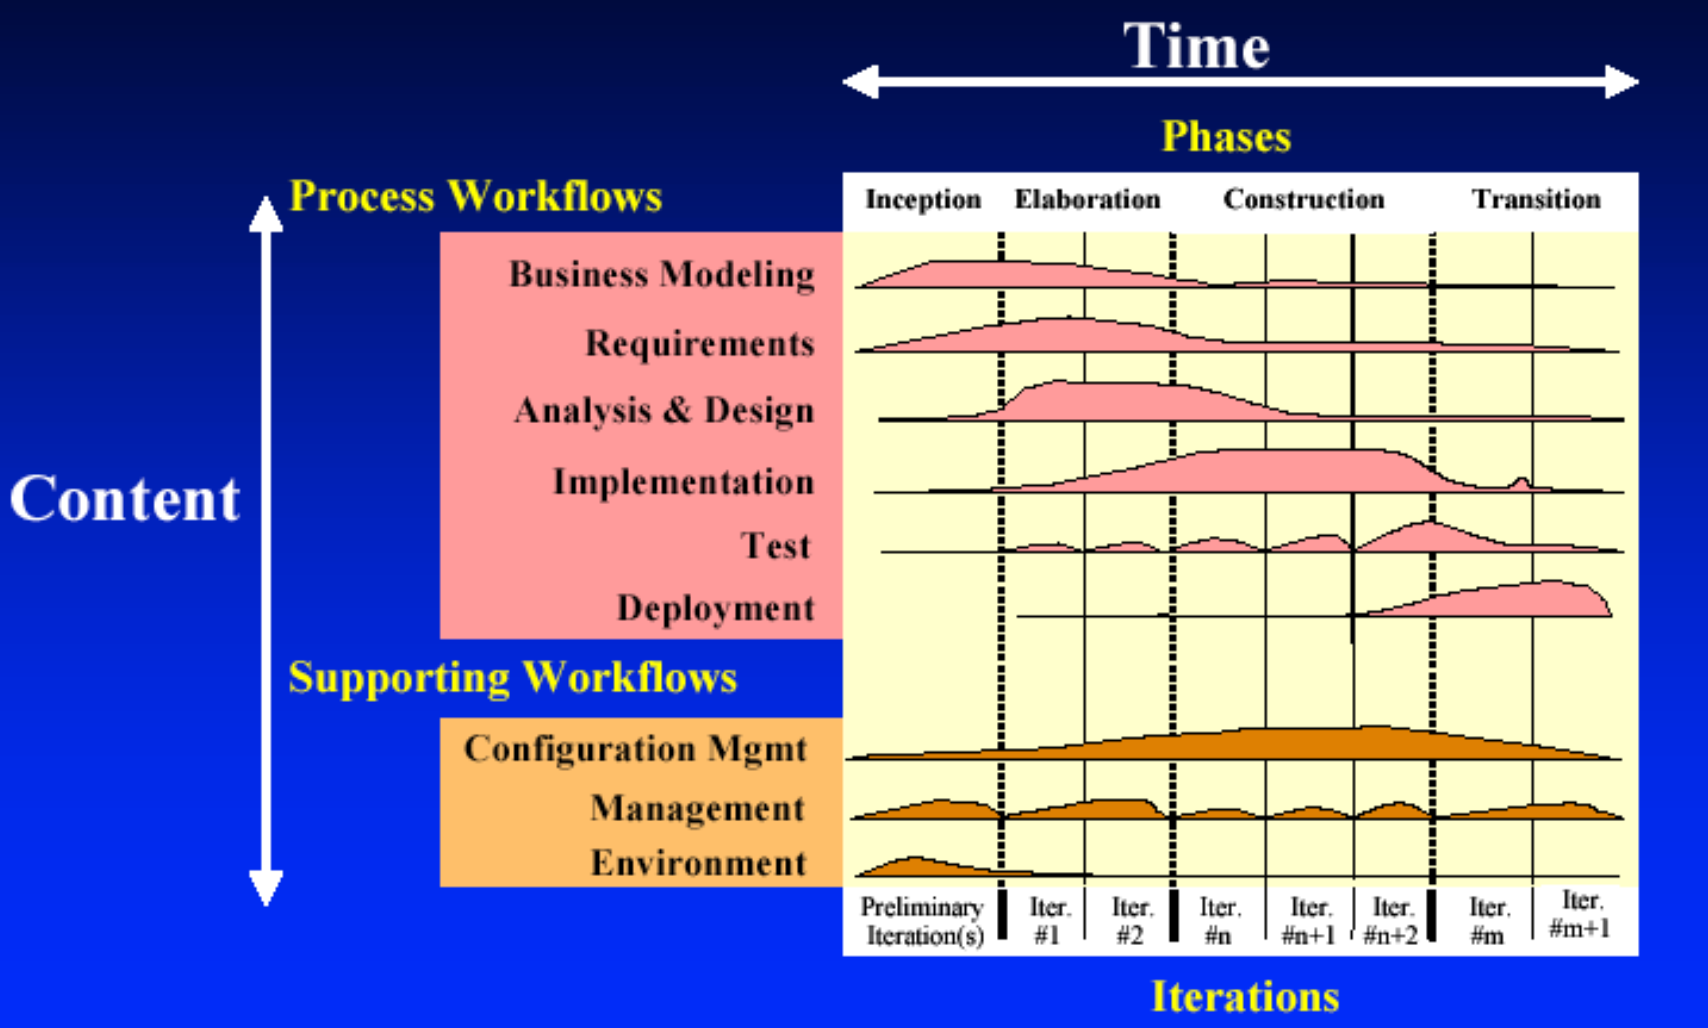
\includegraphics[width=12cm]{RUPplan.png}

\subsection{Iterazioni}

\emph{\textbf{Nota:}} si assume che i requisiti funzionali primari sono tutti quei requisiti con priorità alta e che potrebbero impattare sull'architettura. Al contrario, i requisiti funzionali secondari sono tutti i requisiti con priorità piu bassa e che non hanno impatto sull'architettura.

\begin{center}

\begin{tabular}{ |p{2cm}|p{10cm}|  }
\hline
Nome & Iterazione 1 \\\hline
Fase & Inception \\\hline
Inizio & 20/11/2019 \\\hline
Fine &  1/12/2019 \\\hline
Obbiettivi & 
	\begin{compactitem}
		\item Analisi del problema e prima stesura del documento di Visione
		\item Definire configurazione iniziale del sistema
		\item Analizzare la fattibilità del progetto, dal punto di vista tecnico ed economico
		\item Formulazione di una prima proposta di Contratto
		\item Formulazione documento Glossario
	\end{compactitem}\\\hline
Stato &  Conclusa \\\hline
\end{tabular}
\label{table:1}\newline

\begin{tabular}{ |p{2cm}|p{10cm}|  }
\hline
Nome & Iterazione 2 \\\hline
Fase & Inception \\\hline
Inizio & 15/12/2019 \\\hline
Fine &  18/12/2019 \\\hline
Obbiettivi & 
	\begin{compactitem}
		\item Stesura del piano di progetto
		\item Revisione e aggiornamento della proposta di contratto
		\item Individuare almeno il 50\% dei requisiti funzionali con priorità primaria
	\end{compactitem}\\\hline
Stato &  Conclusa \\\hline
\end{tabular}
\label{table:2}\newline

\begin{tabular}{ |p{2cm}|p{10cm}|  }
\hline
Nome & Iterazione 3 \\\hline
Fase & Inception \\\hline
Inizio & 01/02/2020 \\\hline
Fine &  14/02/2020 \\\hline
Obbiettivi & 
	\begin{compactitem}
		\item Individuare tutti i rimanenti requisiti funzionali con priorità primaria
		\item Individuare almeno il 25\% dei requisiti non funzionali
		\item Descrivere ad alto livello i requisiti individuati
		\item Individuare almeno il 70\% dei rischi e stendere un piano di gestione per ciascun rischio
	\end{compactitem}\\\hline
Stato &  Conclusa \\\hline % Svolgimento 
\end{tabular}
\label{table:3}\newline

\begin{tabular}{ |p{2cm}|p{10cm}|  }
\hline
Nome & Milestone 1\\\hline
Fase & Inception \\\hline
Inizio & 17/02/2020 \\\hline
Fine &  17/02/2020 \\\hline
Obbiettivi & 
	\begin{compactitem}
		\item I requisiti funzionali primari sono stati individuati e descritti correttamente
		\item Almeno il 70\% dei rischi è stato individuato ed è stato creato un piano di gestione per ciascun rischio
		\item Tutte le iterazioni sono state programmate
	\end{compactitem}\\\hline
Stato &  Raggiunta \\\hline
\end{tabular}
\label{table:milestone1}\newline

\begin{tabular}{ |p{2cm}|p{10cm}|  }
\hline
Nome & Iterazione 4 \\\hline
Fase & Elaboration \\\hline
Inizio & 17/02/2020 \\\hline
Fine &  24/02/2020 \\\hline
Obbiettivi & 
	\begin{compactitem}
		\item Iniziare modello di analisi dell'architettura, individuando le classi
		\item Definire il modello dei casi d'uso per il primo 50\% dei requisiti funzionali primari
		\item Individuare 5 requisiti funzionali fondamentali tra i requisiti funzionali primari (che verranno usati per testare l'architettura)
		\item Individuare e descrivere un ulteriore 50\% dei requisiti non funzionali
		\item Individuare un ulteriore 15\% dei rischi e stendere un piano di gestione per ciascun rischio
	\end{compactitem}\\\hline
Stato &  Conclusa \\\hline
\end{tabular}
\label{table:4}\newline

\begin{tabular}{ |p{2cm}|p{10cm}|  }
\hline
Nome & Iterazione 5 \\\hline
Fase & Elaboration \\\hline
Inizio & 26/02/2020 \\\hline
Fine &  03/03/2020  \\\hline
Obbiettivi & 
	\begin{compactitem}
		\item Completare il modello di analisi dell'architettura (completare la descrizione delle classi ed effettuare una suddivisione in package)
		\item Completare il modello dei casi d'uso relativo ai requisiti funzionali primari
		\item Individuare e descrivere i restanti requisiti non funzionali % 100%
		\item Individuare i rischi rimanenti e stendere un piano di gestione per ciascun rischio % 100%
		\item Individuare i primi test sull'architettura e sui requisiti fondamentali
		\item Effettuare una stima dei costi con casi d'uso primari
	\end{compactitem}\\\hline
Stato &  Conclusa \\\hline
\end{tabular}
\label{table:5}\newline

\begin{tabular}{ |p{2cm}|p{10cm}|  }
\hline
Nome & Iterazione 6 \\\hline
Fase & Elaboration \\\hline
Inizio & 05/03/2020 \\\hline
Fine &  14/03/2020  \\\hline
Obbiettivi & 
	\begin{compactitem}		
		\item Iniziare il modello di design dell'architettura
		\item Definire il modello di analisi per i casi d'uso fondamentali individuati
		\item Ampliare i test sull'architettura e sui requisiti fondamentali, in seguito alle scelte di progetto		

	\end{compactitem}\\\hline
Stato &  Programmata \\\hline
\end{tabular}
\label{table:6}\newline

\begin{tabular}{ |p{2cm}|p{10cm}|  }
\hline
Nome & Iterazione 7 \\\hline
Fase & Elaboration \\\hline
Inizio & 15/03/2020 \\\hline
Fine & 25/03/2020 \\\hline
Obbiettivi & 
	\begin{compactitem}
		\item Completare il modello di design dell'architettura
		\item Definire il modello di design per i casi d'uso fondamentali individuati
		\item Implementare l'architettura e i casi d'uso fondamentali individuati
		\item Ultimare i test sull'architettura e sui requisiti fondamentali
	\end{compactitem}\\\hline
Stato &  Programmata \\\hline
\end{tabular}
\label{table:7}\newline

\begin{tabular}{ |p{2cm}|p{10cm}|  }
\hline
Nome & Milestone 2\\\hline
Fase & Elaboration \\\hline
Inizio & 26/03/2020 \\\hline
Fine &  26/03/2020 \\\hline
Obbiettivi & 
	\begin{compactitem}
		\item Tutti i rischi sono stati individuati ed è stato creato un piano di gestione per ciascun rischio
		\item \'E stata effettuata una stima dei costi attendibile
		\item Prendere una decisione Go/NoGo
		\item \'E stata creata una base architetturale coerente con i requisiti ed eseguibile
		\item \'E stato prodotto un modello dei casi d'uso primari sufficientemente dettagliato per iniziare la fase di construction
		\item I casi d'uso fondamentali risultano implementati correttamente con l'architettura prodotta
	\end{compactitem}\\\hline
Stato &  Programmata \\\hline
\end{tabular}
\label{table:milestone2}\newline

\begin{tabular}{ |p{2cm}|p{10cm}|  }
\hline
Nome & Iterazione 8 \\\hline
Fase & Construction \\\hline
Inizio & 27/03/2020 \\\hline
Fine &  04/04/2020  \\\hline
Obbiettivi & 
	\begin{compactitem}

		\item Definire il modello di analisi per il 30\% dei requisiti funzionali primari
		\item Definire il modello di design per il 30\% dei requisiti funzionali primari
		\item Implemetazione e definizione dei test per il 30\% dei requisiti funzionali primari
	\end{compactitem}\\\hline
Stato &  Programmata \\\hline
\end{tabular}
\label{table:8}\newline

\begin{tabular}{ |p{2cm}|p{10cm}|  }
\hline
Nome & Iterazione 9 \\\hline
Fase & Construction \\\hline
Inizio & 05/04/2020 \\\hline
Fine &  12/04/2020  \\\hline
Obbiettivi & 
	\begin{compactitem}
		\item Definire il modello di analisi per un altro 30\% dei requisiti funzionali primari
		\item Definire il modello di design per un altro 30\% dei requisiti funzionali primari
		\item Implementazione e definizione dei test per il 30\% dei requisiti funzionali primari
		
	\end{compactitem}\\\hline
Stato &  Programmata \\\hline
\end{tabular}
\label{table:9}\newline


\begin{tabular}{ |p{2cm}|p{10cm}|  }
\hline
Nome & Iterazione 10 \\\hline
Fase & Construction \\\hline
Inizio & 13/04/2020 \\\hline
Fine &  20/04/2020  \\\hline
Obbiettivi & 
	\begin{compactitem}
		\item Definire il modello di analisi per un altro 30\% dei requisiti funzionali primari
		\item Definire il modello di design per un altro 30\% dei requisiti funzionali primari
		\item Implementazione e definizione dei test per il 30\% dei requisiti funzionali primari
		
		\item individuazione e definizione del modello dei casi d'uso per i requisiti funzionali secondari
	\end{compactitem}\\\hline
Stato &  Programmata \\\hline
\end{tabular}
\label{table:10}\newline

\begin{tabular}{ |p{2cm}|p{10cm}|  }
\hline
Nome & Iterazione 11 \\\hline
Fase & Construction \\\hline
Inizio & 21/04/2020 \\\hline
Fine &  27/04/2020  \\\hline
Obbiettivi & 
	\begin{compactitem}
		\item Definire il modello di analisi per il restante 10\% dei requisiti funzionali primari
		\item Definire il modello di design per il restante 10\% dei requisiti funzionali primari
		\item Implementazione e definizione dei test per il 10\% dei requisiti funzionali primari
		
		\item Definire il modello di analisi dei requisiti funzionali secondari
		\item Definire il modello di design per dei requisiti funzionali secondari
		\item Implementazione e definizione dei test dei requisiti funzionali secondari
		
	\end{compactitem}\\\hline
Stato &  Programmata \\\hline
\end{tabular}
\label{table:11}\newline


\begin{tabular}{ |p{2cm}|p{10cm}|  }
\hline
Nome & Milestone 3\\\hline
Fase & Construction \\\hline
Inizio & 28/04/2020 \\\hline
Fine &  28/04/2020 \\\hline
Obbiettivi & 
	\begin{compactitem}
		\item Sono stati definiti test per ogni funzionalità del sistema
		\item Il sistema e le sue funzionalità implementate hanno superato tutti i test definiti
	\end{compactitem}\\\hline
Stato &  Programmata \\\hline
\end{tabular}
\label{table:milestone3}\newline

\begin{tabular}{ |p{2cm}|p{10cm}|  }
\hline
Nome & Iterazione 12 \\\hline
Fase & Transition \\\hline
Inizio & 29/04/2020 \\\hline
Fine &  2/05/2020  \\\hline
Obbiettivi & 
	\begin{compactitem}
		\item Raccolta Feedback di utilizzo degli utenti
		\item Effettuare correzioni basate sul feedback degli utenti
		\item Creazione degli ultimi test basati sul feedback degli utenti
		\item Creare una release finale
	\end{compactitem}\\\hline
Stato &  Programmata \\\hline
\end{tabular}
\label{table:12}\newline

\begin{tabular}{ |p{2cm}|p{10cm}|  }
\hline
Nome & Milestone 4\\\hline
Fase & Transition \\\hline
Inizio & 03/05/2020 \\\hline
Fine &  03/05/2020 \\\hline
Obbiettivi & 
	\begin{compactitem}
		\item Release finale creata
		\item La release finale supera i test definiti in seguito al feedback degli utenti
	\end{compactitem}\\\hline
Stato &  Programmata \\\hline
\end{tabular}
\label{table:milestone4}\newline


\end{center}

\subsection{Diagramma di Gantt}
\vspace{0.5cm}
\begin{center}
	\hspace*{-2cm}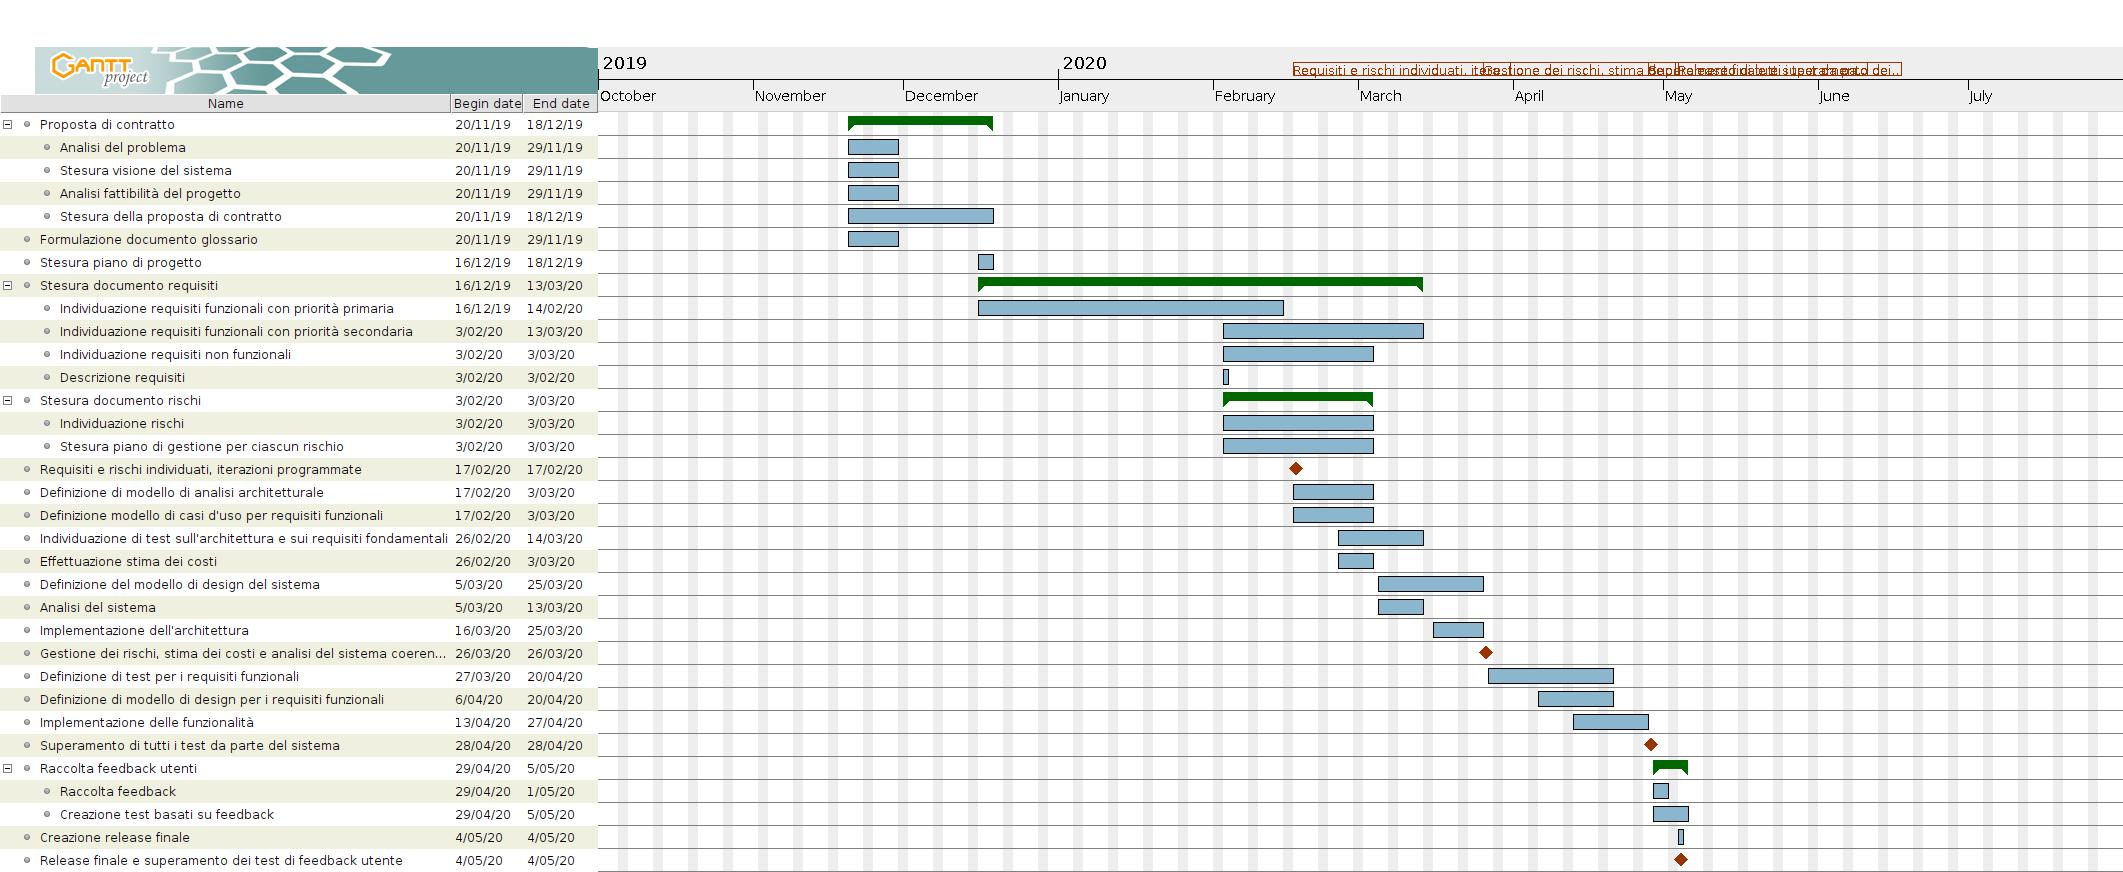
\includegraphics[width=16cm]{Gantt_NexiFy.jpg}
\end{center}
\vspace{2cm}

\clearpage
\noindent{\large \textbf{Revisioni 4-5}} \\ \\
\begin{tabular}{|c | c | c | c|} 
 	\hline
	 Numero & Data & Descrizione \\ [0.5ex] 
	\hline\hline
	1 & 17/12/2019 & Stesura iniziale \\ 
	\hline
	2 & 16/02/2020 & \thead{Specificati meglio gli obiettivi da raggiungere per ogni iterazione,\\e non gli strumenti usati per raggiungerli} \\ 
	\hline
	3 & 26/02/2020 & Revisione del contratto e del piano di progetto \\ 
	\hline
	4 & 14/03/2020 & Specificate meglio attività per implementare l'architettura\\
	\hline
\end{tabular}
\index{Index}

\newpage
\section{\itshape{Analisi dei Requisiti}}


\subsection{Requisiti Funzionali}
\begin{enumerate}
	
	% requisiti relativi agli amministratori

	\item REQ\_F\_CreaAbbonamento
		\begin{itemize}	
			\item Descrizione: permette agli amministratori di creare un nuovo piano di abbonamento (inizialmente con nessun servizio associato)
		\end{itemize}
		\begin{enumerate}[label*=\arabic*.]      
			\item REQ\_F\_EliminaAbbonamento
			\begin{itemize}	
				\item Descrizione: permette agli amministratori di eliminare un piano di abbonamento
			\end{itemize}
			
			\item REQ\_F\_AggiungiServizioAbbonamento
			\begin{itemize}	
				\item Descrizione: permette agli amministratori di aggiungere un certo servizio ad un certo piano di abbonamento
			\end{itemize}
	
			\item REQ\_F\_RimuoviServizioAbbonamento
			\begin{itemize}	
				\item Descrizione: permette agli amministratori di rimuovere un certo servizio ad un certo piano di abbonamento
			\end{itemize}

			\item REQ\_F\_RecuperaServiziAbbonamento
			\begin{itemize}	
				\item Descrizione: permette agli amministratori di recuperare tutti i servizi associati ad un certo abbonamento
			\end{itemize}
	
			\item REQ\_F\_RecuperaServizi
			\begin{itemize}	
				\item Descrizione: permette agli amministratori di recuperare tutti i servizi esistenti
			\end{itemize}
		\end{enumerate}
	\item REQ\_F\_EffettuaPagamento
		\begin{itemize}	
			\item Descrizione: permette agli amministratori di effettuare pagamenti verso utenti che hanno il servizio di pubblicare contenuti
		\end{itemize}

	%requisiti relativi agli utenti
	
	%registrazione
	\item REQ\_F\_EffettuaRegistrazione	
		\begin{itemize}	
			\item Descrizione: permette la registrazione di un nuovo utente (richiedendo vari dati quali nome, cognome, ecc.)
		\end{itemize}
		\begin{enumerate}[label*=\arabic*.]
		\item REQ\_F\_ModificaProfilo
			\begin{itemize}	
				\item Descrizione: permette la modifica del profilo di un utente (può cambiare alcuni dati inseriti in fase di registrazione)
			\end{itemize}

		\item REQ\_F\_EffettuaLogin
			\begin{itemize}	
				\item Descrizione: permette ad un utente registrato di accedere al proprio account
			\end{itemize}

		\item REQ\_F\_EffettuaLogout
			\begin{itemize}	
				\item Descrizione: permette ad un utente di uscire dal proprio account
			\end{itemize}
		\end{enumerate}

	%ricerche
	\item REQ\_F\_RicercaRisorsa
		\begin{itemize}	
			\item Descrizione: permette la ricerca di contenuti coerenti con una stringa digitata dall'utente (eventualmente si può filtrare anche in base al tipo di risorsa: musica, film, ecc.)
		\end{itemize}
		\begin{enumerate}[label*=\arabic*.]
			\item REQ\_F\_RicercaPopolari
			\begin{itemize}
				\item Descrizione: permette la ricerca di contenuti ritenuti popolari in base a vari criteri interni alla piattaforma 
			\end{itemize}	
		\end{enumerate}		

	%abbonamenti
	\item REQ\_F\_SottoscriviAbbonamento
		\begin{itemize}	
			\item Descrizione: permette ad un utente registrato di sottoscrivere un nuovo abbonamento (relativo a un piano di abbonamento esistente)
		\end{itemize}
		\begin{enumerate}[label*=\arabic*.]			
		\item REQ\_F\_DisdiciAbbonamento
			\begin{itemize}	
				\item Descrizione: permette ad un utente registrato di disdire un abbonamento sottoscritto (evitando quindi il prossimo rinnovo, l'abbonamento rimane comunque valido fino alla scadenza)
			\end{itemize}
		\end{enumerate}
		%cambiare abbonamento?? bisogna chiarire...		
	
	%pubblicazione contenuti: l'utente può caricare video (che poi si suddividono in film, serie tv, ecc), canzoni. 
	%per video: serve il video (muto), e le varie tracce audio (diverse lingue) [internamente il sistema genererà un mkv con video e le tracce audio]
	%per musica: serve la traccia audio, un eventuale file dei lyrics (con timestamp per poterlo sincronizzare), un eventuale video musicale (che viene unito all'audio, come per i video)
	
	\item REQ\_F\_CreaProdotto
	\begin{itemize}
		\item Descrizione: permette agli utenti di creare un nuovo prodotto (film/canzone/ecc) da pubblicare sulla piattaforma
	\end{itemize}
	\begin{enumerate}[label*=\arabic*.]
		
		\item REQ\_F\_CreaVideo
		\begin{itemize}
			\item Descrizione: permette agli utenti (che dispongono dell'opportuno servizio) di creare un nuovo video da pubblicare sulla piattaforma
		\end{itemize}
		\begin{enumerate}[label*=\arabic*.]
			\item REQ\_F\_ModificaMetadatiVideo
			\begin{itemize}
				\item Descrizione: permette di modificare i metadati relativi a un video (se è un film o fa parte di una serie tv, genere, titolo, ecc.)
			\end{itemize}
			\item REQ\_F\_AggiungiSottotitoli
			\begin{itemize}
				\item Descrizione: permette di aggiungere un file dei sottotitoli al video
			\end{itemize}
			\item REQ\_F\_CaricaRisorseMultimedialiVideo
			\begin{itemize}
				\item Descrizione: permette di caricare le risorse multimediali per un video (è obbligatorio un file video, possono poi essere aggiunte varie tracce audio in lingue diverse)
			\end{itemize}
		\end{enumerate}
	
		\item REQ\_F\_CreaCanzone
		\begin{itemize}
			\item Descrizione: permette agli utenti (che dispongono dell'opportuno servizio) di creare una nuova canzone da pubblicare sulla piattaforma
		\end{itemize}
		\begin{enumerate}[label*=\arabic*.]
			\item REQ\_F\_ModificaMetadatiCanzone
			\begin{itemize}
				\item Descrizione: permette di modificare i metadati relativi a una canzone (genere, titolo, ecc.)
			\end{itemize}
			\item REQ\_F\_AggiungiLyrics
			\begin{itemize}
				\item Descrizione: permette di aggiungere un file delle lyrics
			\end{itemize}
			\item REQ\_F\_CaricaRisorseMultimedialiCanzone
			\begin{itemize}
				\item Descrizione: permette di caricare le risorse multimediali per una canzone (è obbligatorio un file audio, può essere caricato anche un video multimediale)
			\end{itemize}
		\end{enumerate}	
		
		\item REQ\_F\_CambiaStatoPubblicazione
		\begin{itemize}
			\item Descrizione: permette di modificare lo stato di pubblicazione del prodotto (può essere reso pubbico, oppure lo si può rimettere privato/in bozza)
		\end{itemize}		

	\end{enumerate}
	
	%riproduzione di risorse: chiamiamo riproduciRisorsa, poi questa penserà a usare RiproduciVideo o RiproduciMusica a seconda della risorsa, in RiproduciMusica è necessario trovare la traccia video adeguata, oppure facciamo che la musica in realtà deve essere caricata unitamente al video?
	\item REQ\_F\_RiproduciRisorsa
		\begin{itemize}
			\item Descrizione: riproduce una risorsa multimediale (sia essa video, audio)
		\end{itemize}
    		\begin{enumerate}[label*=\arabic*.]      				
			\item REQ\_F\_RiproduciVideo
				\begin{itemize}
					\item Descrizione: riproduce una risorsa video
				\end{itemize}
			\item REQ\_F\_RiproduciMusica
				\begin{itemize}
					\item Descrizione: riproduce una risorsa musicale, con eventuale traccia video adeguata (lyrics o video musicale)
				\end{itemize}
			
			\item REQ\_F\_PausaRisorsa
				\begin{itemize}
					\item Descrizione: mette in pausa la visualizzazione della risorsa
				\end{itemize}
			
			\item REQ\_F\_SpostaPuntoRiproduzione
				\begin{itemize}
					\item Descrizione: cambia il punto di riproduzione della risorsa (può essere spostata avanti o indietro)
				\end{itemize}		
		\end{enumerate}
		
	%playlist... qualsiasi risorsa, o solo audio? Io direi qualsiasi risorsa e poi se la vede l'utente
	\item REQ\_F\_CreaPlaylist
		\begin{itemize}	
			\item Descrizione: permette ad utenti registrati di creare una playlist (inizialmente vuota)
		\end{itemize}
		\begin{enumerate}[label*=\arabic*.]
		\item REQ\_F\_AggiungiRisorsaAPlaylist
			\begin{itemize}	
				\item Descrizione: permette ad utenti registrati di aggiungere una risorsa a una loro playlist precedentemente creata
			\end{itemize}

		\item REQ\_F\_RimuoviRisorsaDaPlaylist
			\begin{itemize}	
				\item Descrizione: permette ad utenti registrati di rimuovere una risorsa da una loro playlist
			\end{itemize}

		\item REQ\_F\_RiproduciPlaylist
			\begin{itemize}	
				\item Descrizione: riproduce le risorse della playlist, una dopo l'altra
			\end{itemize}
		\end{enumerate}		
	
	%serie tv e album gestite come playlist, che però sono pubbliche
	\item REQ\_F\_CreaSerieTv
		\begin{itemize}	
			\item Descrizione: una serie tv è una playlist di video con dei vincoli: tutti gli episodi devono essere caricati dall'account che crea la serie tv, e un episodio non può appartenere a più serie tv.
		\end{itemize}

	\item REQ\_F\_CreaAlbum
		\begin{itemize}	
			\item Descrizione: un album è una playlist di canzoni con dei vincoli: tutte le canzoni devono essere caricate dall'account che crea l'album.
		\end{itemize}

	%commenti/votazioni
	\item REQ\_F\_VotaRisorsa
		\begin{itemize}	
			\item Descrizione: permette di votare una risorsa (video/musica), agli utenti che l'hanno visionata
		\end{itemize}
		\begin{enumerate}[label*=\arabic*.]
		\item REQ\_F\_CommentaRisorsa
			\begin{itemize}	
				\item Descrizione: permette di commentare una risorsa (video/musica), agli utenti che l'hanno visionata
			\end{itemize}
		\item REQ\_F\_RimuoviCommento
			\begin{itemize}	
				\item Descrizione: permette ad un utente di rimuovere un proprio commento su una risorsa
			\end{itemize}
		\end{enumerate}
		


\end{enumerate}

\subsection{Requisiti Non Funzionali}

\begin{enumerate}
	\item REQ\_NF\_AudioInBackground
		\begin{itemize}
			\item Descrizione: nel caso in cui una musica sia in riproduzione, è necessario continuare a riprodurre la traccia anche quando l'app/sito viene messo in background (inibendo la traccia video)
		\end{itemize}
	
	\item REQ\_NF\_TempoDiRisposta
		\begin{itemize}
			\item Descrizione: la piattaforma deve effettuare le richieste degli utenti in tempi ragionevoli (pochi secondi al massimo), nel caso in cui questo non fosse momentaneamente possibile, è necessario comunicarlo all'utente precisando l'errore
		\end{itemize}

	\item REQ\_NF\_Privacy
		\begin{itemize}
			\item Descrizione: la piattaforma dovrà garantire la riservatezza di dati sensibili degli utenti
		\end{itemize}

	\item REQ\_NF\_Compatibilità
		\begin{itemize}
			\item Descrizione: la piattaforma dovrà essere compatibile su dispositivi Android e iOS (per quanto riguarda l'app), e sui maggiori browser: Firefox, Chrome, Safari (per quanto riguarda la web app)
		\end{itemize}
	
	\item REQ\_NF\_Backup
		\begin{itemize}
			\item Descrizione: la piattaforma deve effettuare backup dei contenuti caricati dagli utenti (insieme ai loro dati), in modo da garantire la disponibilità e la persistenza dei dati
		\end{itemize}

\end{enumerate}

\index{Index}

\newpage
\section{\itshape{Gestione dei Rischi}}
Identificheremo qui i vari rischi per il progetto.\\
Ogni rischio ha una certa probabilità di verificarsi che varia tra: molto bassa, bassa, moderata, alta, molto alta; e provoca dei danni che possono essere: catastrofici, seri, tollerabili, insignificanti.\\
Useremo la tecnica RMMM (Risk Mitigation, Monitoring, Management) per la gestione dei rischi. Per ogni rischio individuato, verrà quindi trovata: 
\begin{itemize}
	\item una strategia di mitigation, per abbassare la probabilità che il rischio si verifichi, e ridurre anche i danni provacati dal rischio
	\item una strategia di monitoring per individuare cambiamenti nella probabilità del rischio
	\item una strategia di management per gestire il rischio, assumendo che questo si sia verificato
\end{itemize}
Inoltre classifichiamo i rischi in base agli aspetti che impattano: progetto, prodotto, business. \\
Identifichiamo i rischi con la convenzione RSC\_\textit{nome}. \\




%\begin{tabular}{|p{2.2cm}|p{9.6cm}| } 
% 	\hline
%	 \textbf{ID} & RSC\_ PerditaDati\\ [0.5ex] 
%	\hline
%	\textbf{Descrizione} & In seguito alla rottura di hard disk dei server, si perdono dati caricati dagli utenti o dati relativi agli utenti \\ 
%	\hline
%	\textbf{Probabilità} &  Molto bassa \\ 
%	\hline
%	\textbf{Impatto} &  Catastrofico \\ 
%	\hline
%	\textbf{Mitigation} & Distribuire i dati su più server ed effettuare backup (anche più di uno) di tutti i dati su server diversi. Sostituire hard disk difettosi. Progettare le varie funzionalità della piattaforma in modo che siano resistenti alle perdite di dati\\ 
%	\hline
%	\textbf{Monitoring} & Monitorare costantemente lo stato degli hard disk dei server, in modo da individuare eventuali problemi \\ 
%	\hline
%	\textbf{Management} & In caso di perdita di dati caricati dagli utenti, comunicarlo agli utenti in modo che possano eventualmente ricaricarli. In caso di dati persi quali informazioni sugli abbonamenti degli utenti, informare gli utenti e cercare di rimborsarli o offrire abbonamenti in omaggio (basandosi sui dati non persi) \\ 
%	\hline
%\end{tabular}

\begin{tabular}{|p{2.2cm}|p{9.6cm}| } 
 	\hline
	 \textbf{ID} & RSC\_ DifficoltàIntegrazioneServizi\\ [0.5ex] 
	\hline
	\textbf{Descrizione} & Diversi servizi esterni usati nella creazione della piattaforma (es: CDN, basi di dati, ecc), non si riescono a integrare come previsto\\ 
	\hline
	\textbf{Aspetto} &  Progetto, Prodotto\\ 
	\hline
	\textbf{Probabilità} &  Moderata\\ 
	\hline
	\textbf{Impatto} &  Serio\\ 
	\hline
	\textbf{Indicatori} & - Una funzionalità di un servizio esterno diventa deprecata\newline
				  - \'E necessario sfruttare più funzionalità del previsto da un servizio esterno \\
	\hline
	\textbf{Trigger} & Le funzionalità di un servizio esterno non possono essere usare insieme alle funzionalità di un altro servizio esterno\\
	\hline
	\textbf{Mitigation} & Prestare attenzione durante la fase di selezione dei servizi esterni, controllando che essi si integrino bene l'uno con l'altro\\ 
	\hline
	\textbf{Monitoring} & Controllare periodicamente eventuali aggiornamenti nei servizi effettuati dalle aziende esterne\\ 
	\hline
	\textbf{Management} & Contattare i fornitori per sapere se esistono soluzioni note per l'integrazione. In caso non esistessero soluzioni note per l'integrazione, si consideri di cambiare uno dei due servizi, in quanto implementare un'integrazione ad-hoc da zero in generale sarebbe più complicato e dispendioso\\ 
	\hline
\end{tabular}

\begin{tabular}{|p{2.2cm}|p{9.6cm}| }
 	\hline
	\textbf{ID} & RSC\_ CambiamentoRequisiti\\ [0.5ex] 
	\hline
	\textbf{Descrizione} & La specifica dei requisiti cambia durante il progetto \\ 
	\hline
	\textbf{Aspetto} &  Progetto\\
	\hline
	\textbf{Probabilità} &  Alta \\ 
	\hline
	\textbf{Impatto} &  Moderato \\ 
	\hline
	\textbf{Indicatori} & L'insieme di alcuni requisiti può portare a casi limite indesiderati\\
	\hline
	\textbf{Trigger} & Stakeholders non soddisfatti dei requisiti\\
	\hline
	\textbf{Mitigation} & Effettuare revisioni periodiche in modo da far emergere tempestivamente possibili cambiamenti nelle specifiche\\%Revisionare attentamente l'analisi dei requisiti all'inizio del progetto, in modo da abbassare la probabilità di grandi cambiamenti.\\ 
	\hline
	\textbf{Monitoring} & Durante le revisioni e l'analisi dei requisiti, immaginare situazioni limite che potrebbero verificarsi\\%Effettuare revisioni periodiche in modo da far emergere tempestivamente possibili cambiamenti nelle specifiche\\ 
	\hline
	\textbf{Management} & Se le modifiche ai requisiti non comportano un grande ritardo nel progetto, o si tratta di requisiti di alta priorità, allora adattare il progetto ai nuovi requisiti. Se dopo aver aggiunto i nuovi requisiti la durata del progetto supera di molto quella precedentemente prevista, eliminare requisiti secondari per restare nei tempi \\ 
	\hline
\end{tabular}


\clearpage
\begin{tabular}{|p{2.2cm}|p{9.6cm}| }
 	\hline
	\textbf{ID} & RSC\_ IndisponibilitàPersonale\\ [0.5ex] 
	\hline
	\textbf{Descrizione} & Alcuni elementi del personale potrebbero essere indisponibili in alcuni periodi del progetto\\ 
	\hline
	\textbf{Aspetto} &  Progetto \\
	\hline
	\textbf{Probabilità} &  Alta \\ 
	\hline
	\textbf{Impatto} &  Tollerabile \\ 
	\hline
	\textbf{Indicatori} & Malcontento del personale\\
	\hline
	\textbf{Trigger} & -\\
	\hline
	\textbf{Mitigation} & Fare una previsione di eventuali giorni di assenza mentre si pianifica lo sviluppo oltre che incoraggiare i dipendenti a comunicare in anticipo eventuali indisponibilità già previste (tipicamente indisponibilità non dovute a malattie) \\ 
	\hline
	\textbf{Monitoring} & Mantenere una comunicazione tra dipendenti e resto dell'azienda, per venire a conoscenza il prima possibile di indisponibilità e monitorare periodicamente quanto prodotto effettivamente dai membri rispetto quello che avrebbero dovuto produrre secondo il piano in modo da rilevare ritardi\\ 
	\hline
	\textbf{Management} & Se l'indisponibilità è per un breve periodo, distribuire il lavoro del personale assente sugli altri dipendenti. Se l'indisponibilità si protrae troppo a lungo, assumere nuovi dipendenti per un certo periodo o addirittura valutare una riprogrammazione delle scadenza\\ 
	\hline
\end{tabular}


\begin{tabular}{|p{2.2cm}|p{9.6cm}| }
 	\hline
	\textbf{ID} & RSC\_ CasiD'UsoErrati\\ [0.5ex] 
	\hline
	\textbf{Descrizione} & I requisiti non vengono compresi nella realizzazione dei casi d'uso.\\ 
	\hline
	\textbf{Aspetto} &  Progetto\\
	\hline
	\textbf{Probabilità} &  Bassa \\ 
	\hline
	\textbf{Impatto} &  Serio \\ 
	\hline
	\textbf{Indicatori} & Cambiamento nei requisiti\\
	\hline
	\textbf{Trigger} & Incomprensione nell'interpretazione dei requisiti\\
	\hline
	\textbf{Mitigation} & Revisionare attentamente l'analisi dei requisiti prima di definire i casi d'uso.\\ 
	\hline
	\textbf{Monitoring} & Effettuare revisioni periodiche in modo da far emergere tempestivamente possibili fraintendimenti delle specifiche\\ 
	\hline
	\textbf{Management} & Ridefinire i casi d'uso in modo da renderli coerenti con i requisiti corretti. Se dopo aver modificato i casi d'uso la durata del progetto supera di molto quella precedentemente prevista, eliminare requisiti secondari per restare nei tempi \\ 
	\hline
\end{tabular}
\clearpage
\begin{tabular}{|p{2.2cm}|p{9.6cm}| }
	\hline
   \textbf{ID} & RSC\_ TecnologiaObsoleta\\ [0.5ex] 
   \hline
   \textbf{Descrizione} & Durante l'implementazione del progetto, le tecnologie che si intendono utilizzare diventano obsolete \\ 
   \hline
   \textbf{Aspetto} &  Progetto \\
   \hline
   \textbf{Probabilità} & Moderata\\ 
   \hline
   \textbf{Impatto} & Tollerabile\\
	\hline
	\textbf{Indicatori} & - Piattaforme con le stesse difficoltà di Nexify si preparano ad un cambio di tecnologia\\
	\hline
	\textbf{Trigger} & - Una tecnologia diversa da quella adottata si consolida come la più adatta\\
   \hline
   \textbf{Mitigation} & Scegliere, al momento dello sviluppo iniziale, tecnologie aggiornate e che abbiano dimostrato di essere affidabili in altri progetti \\ 
   \hline
   \textbf{Monitoring} & Tenere traccia periodicamente delle tecnologie esistenti, e di possibili nuovi aggiornamenti o cambiamenti che avvengono \\ 
   \hline
   \textbf{Management} & Effettuare un’analisi per capire se la tecnologia originale è ancora adatta allo svolgimento del compito per cui è stata scelta. In caso negativo, deve essere sostituita con una tecnologia più adatta.\\ 
   \hline
\end{tabular}


\begin{tabular}{|p{2.2cm}|p{9.6cm}| }
	\hline
   \textbf{ID} & RSC\_ DimensioneSoftwareSottostimata\\ [0.5ex] 
   \hline
   \textbf{Descrizione} & La dimensione del software da produrre viene sottostimata \\ 
   \hline
   \textbf{Aspetto} &  Progetto \\
   \hline
   \textbf{Probabilità} & Moderata\\ 
   \hline
   \textbf{Impatto} & Serio\\
	\hline
	\textbf{Indicatori} & - Le stime iniziali sulla dimensione del software si rivelano non attendibili \\
	\hline
	\textbf{Trigger} & - Le stime correnti portano a superare la scadenza dell'iterazione corrente\\
   \hline
   \textbf{Mitigation} & Svolgere in maniera accurata le fase di analisi e pianificazione del progetto, in modo da stimare una dimensione il più vicino possibile a quella reale. Inoltre per ogni iterazione aggiungere dei giorni aggiuntivi per fare fronte a eventuali ritardi dovuti a stime sbagliate \\ 
   \hline
   \textbf{Monitoring} & Durante lo sviluppo, controllare periodicamente che la dimensione del software rimanga contenuta, in base a quanto è stato pianificato nelle fasi iniziali\\ 
   \hline
   \textbf{Management} & Qualora, durante lo sviluppo, il software dovesse superare la dimensione prestabilita per quello stadio, si deve effettuare una nuova stima che tenga conto delle nuove informazioni acquisite. Successivamente si deve rivedere la pianificazione del progetto, eventualmente apportando modifiche laddove la dimensione del software risulta maggiore di quella stimata inizialmente \\ 
   \hline
\end{tabular}

\begin{tabular}{|p{2.2cm}|p{9.6cm}| } 
 	\hline
	 \textbf{ID} & RSC\_ SovraccaricoCDN\\ [0.5ex] 
	\hline
	\textbf{Descrizione} & Le richieste effettuate dagli utenti superano il carico massimo sopportabile dalla CDN \\ 
	\hline
   	\textbf{Aspetto} &  Prodotto \\
	\hline
	\textbf{Probabilità} &  Moderata \\ 
	\hline
	\textbf{Impatto} &  Tollerabile \\ 
	\hline
	\textbf{Indicatori} & - Il numero di richieste di contenuti contemporanee aumenta \newline
						  - Guasti della CDN\\
	\hline
	\textbf{Trigger} & - Il numero di richieste ad un nodo è maggiore delle richieste gestibili\newline
					   - Non ci sono abbastanza nodi per gestire la richieste in una certa area\\
	\hline
	\textbf{Mitigation} & Viene sottoscritta una SLA che impone delle penali e permette di rescindere il contratto nel caso in cui la qualit\'a del servizio non venga rispettata. Inoltre si definiscono nella SLA i tempi di risoluzione del disservizio ed estensione delle capacit\'a della CDN. \\ 
	\hline
	\textbf{Monitoring} & Osservare periodicamente il numero di richieste ricevute, e i file di log dei nodi della CDN, in modo da individuare possibili sovraccarichi. Inoltre si valutano eventuali segnalazioni degli utenti riguardanti la qualit\'a del servizio\\ 
	\hline
	\textbf{Management} & Nel caso in cui la qualit\'a del servizio della CDN non rispettasse la qualit\'a definita nel contratto si richieder\'a un'incremento delle prestazioni. Se il fornitore del servizio non riuscisse a risolvere il problema si può rescindere il contratto e riscuorete le penali. \\ 
	\hline
\end{tabular}


\begin{tabular}{|p{2.2cm}|p{9.6cm}| } 
 	\hline
	 \textbf{ID} & RSC\_ DegradoQualitàContenuti\\ [0.5ex] 
	\hline
	\textbf{Descrizione} & Contenuti amatoriali di scarsa qualità abbondano sulla piattaforma, portando a un degrado della qualità dei contenuti offerti. \\ 
	\hline
   	\textbf{Aspetto} &  Prodotto \\
	\hline
	\textbf{Probabilità} &  Bassa \\ 
	\hline
	\textbf{Impatto} &  Tollerabile \\ 
	\hline
	\textbf{Indicatori} & - L'abbasssamento della quota di sottoscrizione di abbonamenti abilitati alla pubblicazione \newline
						  - Diminuzione della popolarit\'a della piattaforma\\
	\hline
	\textbf{Trigger} & - La quota di iscrizione ad abbonamenti partner permette l'iscrizione a pubblicatori non affidabili\newline
					   - La piattaforma non è popolare e ai pubblicatori di alto calibro non conviene pubblicare contenuti (affidabili) sulla piattaforma\\
	\hline
	\textbf{Mitigation} & Scegliere attentamente i costi che gli utenti devono pagare per poter pubblicare contenuti. \newline
						  Investire nella pubblicit\'a della piattaforma \\ 
	\hline
	\textbf{Monitoring} & Controlli periodici sui contenuti presenti sulla piattaforma. \newline
						  Controllare il calibro dei pubblicatori iscritti alla piattaforma \\ 
	\hline
	\textbf{Management} & Aumentare il prezzo richiesto per abilitare la pubblicazione di prodotti \newline
						  Fare pubblicit\'a per nuovi abbonamenti\\ 
	\hline
\end{tabular}


\begin{tabular}{|p{2.2cm}|p{9.6cm}| }
 	\hline
	\textbf{ID} & RSC\_ DurataSottostimata\\ [0.5ex] 
	\hline
	\textbf{Descrizione} & La durata dell'iterazione corrente viene sottostimata \\ 
	\hline
	\textbf{Aspetto} &  Progetto \\
	\hline
	\textbf{Probabilità} & Basso\\ 
	\hline
	\textbf{Impatto} & Serio\\
	\hline
	\textbf{Indicatori} & - Problemi emersi durante svoglimento del lavoro prefissato\\
	\hline
	\textbf{Trigger} & - La gestione dei problemi sorti provoca uno slittamento dei tempi che non permette di ultimare il lavoro prefissato nell'iterazione corrente\\
	\hline
	\textbf{Mitigation} & Lasciare qualche giorno in più del previsto in ogni iterazione, in modo da far fronte a eventuali errori di stima per una certa iterazione\\ 
	\hline
	\textbf{Monitoring} & Esaminare periodicamente l'andamento dell'iterazione corrente, in modo da individuare potenziali situazioni che portano a superare la durata stimata dell'iterazione\\ 
	\hline
	\textbf{Management} & Se è la prima iterazione che è stata sottostimata, si può distribuire il lavoro in eccesso sull'iterazione successiva, in quanto è improbabile aver sottostimato due iterazioni consecutive. Se è la seconda iterazione di fila che è stata sottostimata, considerare la rimozione di requisiti meno importanti, in quanto si accumulerebbe troppo lavoro continuando a rimandare sulle fasi successive \\ 
	\hline
\end{tabular}


\begin{tabular}{|p{2.2cm}|p{9.6cm}| }
 	\hline
	\textbf{ID} & RSC\_ RiduzioneBudget\\ [0.5ex] 
	\hline
	\textbf{Descrizione} & Il budget disponibile viene ridotto durante il progetto\\ 
	\hline
	\textbf{Aspetto} &  Business\\
	\hline
	\textbf{Probabilità} & Molto basso\\ 
	\hline
	\textbf{Impatto} & Catastrofico\\
	\hline
	\textbf{Indicatori} & - Introduzione di costi non previsti \newline
						  - Riduzione dei finanziamenti\\
	\hline
	\textbf{Trigger} & - Nuovi costi emergono rispetto a quelli precedentemente stabiliti eccedendo una certa soglia\newline
					   - L'ammontare dei finanziamenti ricevuti diminuisce rispetto al minimo previsto inizialmente\\
	\hline
	\textbf{Mitigation} & Richiedere inizialmente un budget leggermente più alto del necessario, in modo da coprire eventuali, piccole, riduzioni\\
	\hline
	\textbf{Monitoring} & Controllare periodicamente che l'avanzamento del progetto segua i costi previsti, e sfruttare eventuali condizioni che portano a risparmio\\ 
	\hline
	\textbf{Management} & Ridimensionare il progetto in base al nuovo budget, rimuovendo le funzionalità meno importanti\\ 
	\hline
\end{tabular}

\renewcommand\theadfont{}

\newpage
\noindent{\large \textbf{Revisioni 7}} \\ \\
\begin{tabular}{|c | c | c | c|} 
 	\hline
	 Numero & Data & Descrizione \\ [0.5ex] 
	\hline\hline
	1 & 07/02/2020 & Stesura iniziale \\ 
	\hline
	2 & 16/02/2020 & Modificato monitoring e management di REQ\_M\_DurataSottostimata \\
	\hline
	3 & 15/03/2020 & Aggiunti trigger e indicatori di rischio \\
	\hline
\end{tabular}
\index{Index}

\newpage
\section{\itshape{Modello degli Use-Case}}
\setlength{\arrayrulewidth}{.5mm}
\setlength{\tabcolsep}{5pt}
\renewcommand{\arraystretch}{2}
\renewcommand{\labelenumii}{\theenumii}
\renewcommand{\theenumii}{\theenumi.\arabic{enumii}.}

\subsection{Introduzione}
La seguente sezione mira all'identificazione dei casi d'uso presenti nel progetto. Di seguito vengono identificati oltre ai casi d'uso, anche gli attori coinvolti nel loro utilizzo.
Lo scopo principale del documento, è quello di avere un riferimento sui casi d'uso leggibile da chiunque, anche a personale non interno al progetto. Questo è utile al fine di permettere a tutti una comprensione e quindi una discussione sui casi d'uso.

\subsection{Legenda}
\large{\textbf{Attori}} \\
\begin{itemize}[]
	\item \textbf{ID}: rappresenta l'identificatore univoco di un attore. La sintassi è del tipo A\_X dove X è una stringa di interi separati da punto che rappresenta la gerarchia di relazioni padre-figlio.
	\item \textbf{Nome}: nome dell'attore, deve essere comunque univoco e deve dare una prima idea di cosa rappresenta quel preciso attore.
	\item \textbf{Genitore}: indica l'identificatore del primo antenato nella gerarchia degli attori.
	\item \textbf{Livello}: indica il grado di rilevanza dell'attore all'interno dell'intero sistema. Può assumere il valore di {Primario, Secondario, Di Supporto}.
	\item \textbf{Tipologia}: classifica l'attore in {Umano, Sistema}
	\item \textbf{Descrizione}: descrive brevemente cosa rappresenta all'interno del sistema l'attore.\
\end{itemize}


\noindent \large{\textbf{Use Case}} \\
\begin{itemize}[]
	\item \textbf{ID}: identificativo univoco del caso d'uso, è della forma UC\_X dove X è una stringa di interi separati da punto che rappresenta la gerarchia di relazioni padre-figlio.
	\item \textbf{Categoria}: Macroarea di appartenza della funzionalità. Può assumere i valori {User, Subscriptions, Management}
	\item \textbf{Nome}: Nome identificativo del caso d'uso, serve anche per dare un'idea del tipo di attività.
	\item \textbf{Priorità}: Livello di priorità del caso d'uso. Può assumere i valori {High, Medium, Low}. 
	\item \textbf{Attori}: Lista di identificativi degli attori coinvolti nel caso d'uso.
	\item \textbf{Descrizione}: Breve descrizione della funzione svolta dal caso d'uso.
	\item \textbf{Input}: Lista di cosa riceve in input il caso d'uso (se non indicato, si assume che non riceve niente in input)
	\item \textbf{Output}: Lista di cosa restituisce il caso d'uso (se non è indicato, si assume che non restituisce niente)
	\item \textbf{Pre-condizioni}: Condizioni che devono essere verificate prima che il caso d'uso inizi, altrimenti non potrà essere svolto.
	\item \textbf{Post-condizioni}: Condizioni che devono essere verificate subito dopo l'esecuzione del caso d'uso.
	\item \textbf{Flusso}: Passi logici eseguiti dal caso d'uso per ottenere il risultato desiderato.
	%\item \textbf{Flusso Alternativo}: 

\end{itemize}

% ============================== ATTORI ====================================

\subsection{Specifica Attori}

\begin{center}

\begin{tabular}{ |p{2cm}|p{10cm}|  }
\hline
ID & A\_1 \\\hline
Nome & Utente\\\hline
Genitore & - \\\hline
Livello &  Primario \\\hline
Tipologia & Umano \\\hline
Descrizione &  L' Utente è il ruolo assunto da tutti coloro che usufruiranno del servizio di streaming offerto dalla piattaforma. \\\hline
\end{tabular}
\label{table_attore:1}\newline

\begin{tabular}{ |p{2cm}|p{10cm}|  }
\hline
ID & A\_1.1 \\\hline
Nome & UtenteNonAutenticato\\\hline
Genitore & A\_1 \\\hline
Livello &  Primario \\\hline
Tipologia & Umano \\\hline
Descrizione &  Questo ruolo è assunto da tutti coloro che utilizzano la piattaforma senza aver effettuato l'accesso ad un profilo utente e che quindi avranno accesso solo a determinate funzionalità \\\hline
\end{tabular}
\label{table_attore:1.1}\newline

\begin{tabular}{ |p{2cm}|p{10cm}|  }
\hline
ID & A\_1.2 \\\hline
Nome & UtenteAutenticato\\\hline
Genitore & A\_1 \\\hline
Livello &  Primario \\\hline
Tipologia & Umano \\\hline
Descrizione &  Questo ruolo è assunto da tutti gli utenti che hanno sottoscritto un contratto con la piattaforma e si sono autenticati in fase di accesso ad essa. \\\hline
\end{tabular}
\label{table_attore:1.2}\newline

\begin{tabular}{ |p{2cm}|p{10cm}|  }
\hline
ID & A\_1.3 \\\hline
Nome & Staff\\\hline
Genitore & A\_1\\\hline
Livello &  Primario \\\hline
Tipologia & Umano \\\hline
Descrizione &  Rappresenta il ruolo di staff della piattaforma \\\hline
\end{tabular}
\label{table_attore:1.3}\newline

\begin{tabular}{ |p{2cm}|p{10cm}|  }
\hline
ID & A\_1.3.1 \\\hline
Nome & ManagerAbbonamenti\\\hline
Genitore & A\_1.3\\\hline
Livello &  Primario \\\hline
Tipologia & Umano \\\hline
Descrizione &  Rappresenta il ruolo di chi gestisce i servizi offerti dalla piattaforma \\\hline
\end{tabular}
\label{table_attore:1.3.1}\newline

\begin{tabular}{ |p{2cm}|p{10cm}|  }
\hline
ID & A\_1.3.2 \\\hline
Nome & ManagerPagamenti\\\hline
Genitore & A\_1.3\\\hline
Livello &  Primario \\\hline
Tipologia & Sistema \\\hline
Descrizione &  Rappresenta il sistema di gestione dei pagamenti verso i partner \\\hline
\end{tabular}
\label{table_attore:1.3.1}\newline

\begin{tabular}{ |p{2cm}|p{10cm}|  }
\hline
ID & A\_1.3.3 \\\hline
Nome & ManagerSegnalazioni\\\hline
Genitore & A\_1.3\\\hline
Livello &  Primario \\\hline
Tipologia & Umano \\\hline
Descrizione &  Rappresenta il ruolo di chi gestisce tutte le segnalazioni verso prodotti o utenti \\\hline
\end{tabular}
\label{table_attore:1.3.1}\newline

\begin{tabular}{ |p{2cm}|p{10cm}|  }
\hline
ID & A\_2 \\\hline
Nome & Pagamento\\\hline
Genitore & - \\\hline
Livello &  Primario \\\hline
Tipologia & Sistema \\\hline
Descrizione &  Rappresenta il sistema di pagamento esterno al sistema della piattaforma \\\hline
\end{tabular}
\label{table_attore:2}\newline

\begin{tabular}{ |p{2cm}|p{10cm}|  }
\hline
ID & A\_3 \\\hline
Nome & Database\\\hline
Genitore & - \\\hline
Livello &  Primario \\\hline
Tipologia & Sistema \\\hline
Descrizione &  Rappresenta il sistema usato per la memorizzazione di informazioni. \\\hline
\end{tabular}
\label{table_attore:3}\newline

\begin{tabular}{ |p{2cm}|p{10cm}|  }
\hline
ID & A\_4 \\\hline
Nome & CDN\\\hline
Genitore & - \\\hline
Livello &  Primario \\\hline
Tipologia & Sistema \\\hline
Descrizione &  Rappresenta il sistema di distribuzione dei contenuti. \\\hline
\end{tabular}
\label{table_attore:4}\newline

\begin{tabular}{ |p{2cm}|p{10cm}|  }
\hline
ID & A\_5 \\\hline
Nome & Time\\\hline
Genitore & - \\\hline
Livello &  Primario \\\hline
Tipologia & Sistema \\\hline
Descrizione &  Rappresenta la componente responsabile dello scheduling delle operazioni \\\hline
\end{tabular}
\label{table_attore:5}\newline


\end{center}

%==== gestione errori di default ====
\subsection{Gestione Fallimenti}
Specifichiamo qui le politiche standard di gestione dei fallimenti di sistemi esterni. Se negli use case non viene specificato esplicitamente come gestire un fallimento di questi sistemi, si assume che entrino in atto queste politiche.

\begin{tabular}{ |p{2cm}|p{10cm}|  }
\hline
ID & F\_1\\\hline
Nome & F\_FallimentoDatabase\\\hline
Attore & Database\\\hline
Descrizione & una richiesta al database produce un errore, e non viene quindi restituito il risultato richiesto\\\hline
Gestione &  La procedura che ha effettuato la richiesta al database viene abortita, riportando un messaggio di errore \\\hline
\end{tabular}
\label{table_fail:1}\newline

\begin{tabular}{ |p{2cm}|p{10cm}|  }
\hline
ID & F\_2\\\hline
Nome & F\_FallimentoCDN\\\hline
Attore & CDN\\\hline
Descrizione & una richiesta alla CDN produce un errore\\\hline
Gestione &  La procedura che ha effettuato la richiesta alla CDN viene abortita, riportando un messaggio di errore \\\hline
\end{tabular}
\label{table_fail:2}\newline

% ================ USE CASE CHE VANNO BENE ===========
\subsection{Specifica Use Case}

\begin{center}

%======= UC relativi ai requisiti funzionali 1. ==========
\begin{table}[bp]
    \centering
    \addtolength{\leftskip} {-2cm}
\begin{tabular}{ |p{2.6cm}|p{13cm}|  }
\hline
ID & UC\_\lastUC \\\hline
Categoria & Management\\\hline
Nome & UC\_CreaAbbonamento\\\hline
Priorità & High \\\hline
Attori &  ManagerAbbonamenti \\\hline
Descrizione & Crea un nuovo piano di abbonamento senza nessun servizio associato.\\\hline
Pre-condizioni &  \'E possibile creare un nuovo piano di abbonamento\\\hline
Post-condizioni &  Esiste un piano di abbonamento con il nome fornito dal manager degli abbonamenti\\\hline
Flusso &  	\begin{enumerate}
			\item Il manager degli abbonamenti richiede la creazione di un nuovo piano di abbonamento;
			\item Il sistema richiede al manager degli abbonamenti il nome, il prezzo e la durata del nuovo piano di abbonamento;
			\item Il manager degli abbonamenti fornisce i dati;
			\item Il sistema valida gli input, e:
				\begin{enumerate}[  ]
				\item \textbf{\# alt1}: Se non avvengono errori durante la validazione:
					\begin{enumerate}[label*=\arabic*.]
					\item Il sistema ricerca se esistono altri piani di abbonamento con il nome inserito:
						\begin{enumerate}[label*=\arabic*.]
						\item \textbf{\# alt1}: Se non esistono altri piani di abbonamento con il nome inserito: il piano di abbonamento viene creato, con i dati inseriti dal manager degli abbonamenti, la lista dei servizi inizialmente vuota e inizialmente non sottoscrivibile
						\item \textbf{\# alt2}: Se esistono altri piani di abbonamento con il nome inserito: la creazione viene annullata e viene comunicato al manager degli abbonamenti che esiste già un piano di abbonamento con il nome inserito	
						\end{enumerate}
					\end{enumerate}
				\item \textbf{\# alt2}: Se avvengono errori durante la validazione: il piano di abbonamento non viene creato e l'errore viene comunicato al manager degli abbonamenti
				\end{enumerate}
			
			\end{enumerate}\\\hline
\end{tabular}
\label{table_use_case:\lastUC}\newline
\end{table}

\begin{table}[bp]
    \centering
    \addtolength{\leftskip} {-2cm}
\begin{tabular}{ |p{2.6cm}|p{13cm}|  }
\hline
ID & UC\_\nextUC \\\hline
Categoria & Management\\\hline
Nome & UC\_RecuperaAbbonamentiEsistenti\\\hline
Priorità & High \\\hline
Attori &  Staff \\\hline
Descrizione & Recupera tutti i piani di abbonamento attualmente esistenti.\\\hline
Input &  - \\\hline
Output &  Tutti i piani di abbonamento esistenti\\\hline
Pre-condizioni &  Nessuna \\\hline
Post-condizioni &  Tutti i piani di abbonamento esistenti vengono restituiti\\\hline
Flusso &  	\vspace{-5mm} \begin{enumerate}
			\item Il sistema effettua una richiesta al sistema Database per richiedere tutti i piani di abbonamento
			\item viene restituita la lista dei piani di abbonamento trovati
		\end{enumerate}\\\hline
\end{tabular}
\label{table_use_case:\lastUC}\newline
\end{table}

\begin{table}[bp]
    \centering
    \addtolength{\leftskip} {-2cm}
\begin{tabular}{ |p{2.6cm}|p{13cm}|  }
\hline
ID & UC\_\nextUC \\\hline
Categoria & Management\\\hline
Nome & UC\_RecuperaServizi\\\hline
Priorità & High \\\hline
Attori &  Staff \\\hline
Descrizione & Permette di recuperare la lista di tutti i servizi esistenti.\\\hline
Input &  - \\\hline
Output &  Tutti i servizi esistenti\\\hline
Pre-condizioni &  Nessuna.\\\hline
Post-condizioni &  Nessuna\\\hline
Flusso &  	\vspace{-5mm} \begin{enumerate}
			\item Il sistema effettua una richiesta al sistema Database per richiedere tutti i servizi
			\item viene restituita la lista dei servizi trovati
		\end{enumerate}\\\hline
\end{tabular}
\label{table_use_case:\lastUC}\newline
\end{table}

\begin{table}[bp]
    \centering
    \addtolength{\leftskip} {-2cm}
\begin{tabular}{ |p{2.6cm}|p{13cm}|  }
\hline
ID & UC\_\nextUC \\\hline
Categoria & Management\\\hline
Nome & UC\_DisattivaAbbonamento\\\hline
Priorità & High \\\hline
Attori &  ManagerAbbonamenti \\\hline
Descrizione & Rende non più sottoscrivibile un piano di abbonamento esistente.\\\hline
Pre-condizioni &  Il manager ha indicato la disattivazione di uno specifico piano di abbonamento\\\hline
Post-condizioni &  Il piano di abbonamento specificato non è più sottoscrivibile\\\hline
Flusso &  	\vspace{-5mm} \begin{enumerate}
		\item Il sistema richiede al Database di salvare che il piano di abbonamento specificato non è più sottoscrivibile\newline
		\end{enumerate}\\\hline
\end{tabular}
\label{table_use_case:\lastUC}\newline
\end{table}

\begin{table}[bp]
    \centering
    \addtolength{\leftskip} {-2cm}
\begin{tabular}{ |p{2.6cm}|p{13cm}|  }
\hline
ID & UC\_\nextUC \\\hline
Categoria & Management\\\hline
Nome & UC\_AttivaAbbonamento\\\hline
Priorità & High \\\hline
Attori &  ManagerAbbonamenti \\\hline
Descrizione & Rende sottoscrivibile un piano di abbonamento esistente.\\\hline
Pre-condizioni &  Il manager ha indicato l'attivazione di uno specifico piano di abbonamento\\\hline
Post-condizioni &  Il piano di abbonamento specificato è sottoscrivibile\\\hline
Flusso &  	\vspace{-5mm} \begin{enumerate}
		\item Il sistema richiede al Database di salvare che il piano di abbonamento specificato è sottoscrivibile\newline
		\end{enumerate}\\\hline
\end{tabular}
\label{table_use_case:\lastUC}\newline
\end{table}


\begin{table}[bp]
    \centering
    \addtolength{\leftskip} {-2cm}
\begin{tabular}{ |p{2.6cm}|p{13cm}|  }
\hline
ID & UC\_\nextUC \\\hline
Categoria & Management\\\hline
Nome & UC\_AggiungiServizioAbbonamento\\\hline
Priorità & High \\\hline
Attori &  ManagerAbbonamenti \\\hline
Descrizione & Permette di aggiungere un servizio all'insieme dei servizi disponibili in un piano di abbonamento.\\\hline
Pre-condizioni & Il manager ha indicato uno specifico piano di abbonamento al quale vuole aggiungere un servizio\\\hline
Post-condizioni & Un nuovo servizio viene aggiunto al piano di abbonamento indicato\\\hline
Flusso &  	\vspace{-5mm} \begin{enumerate}
		\item Il sistema mostra la lista dei servizi che possono essere aggiunti al piano di abbonamento indicato		
			\begin{enumerate}[label*=\arabic*.]
			\item (UC\_3) Il sistema recupera tutti i servizi disponibili
			\item (UC\_8) Il sistema recupera tutti i servizi associati al piano di abbonamento indicato
			\item La lista dei servizi sarà la differenza tra il primo e il secondo insieme calcolati
			\end{enumerate}
		\item Il manager degli abbonamenti sceglie dalla lista, il servizio da aggiungere al piano di abbonamento
		\item Il sistema richiede al Database di aggiungere il servizio scelto alla lista dei servizi per il piano di abbonamento indicato
		\end{enumerate}\\\hline
\end{tabular}
\label{table_use_case:\lastUC}\newline
\end{table}

\begin{table}[bp]
    \centering
    \addtolength{\leftskip} {-2cm}
\begin{tabular}{ |p{2.6cm}|p{13cm}|  }
\hline
ID & UC\_\nextUC \\\hline
Categoria & Management\\\hline
Nome & UC\_RimuoviServizioAbbonamento\\\hline
Priorità & High \\\hline
Attori &  ManagerAbbonamenti \\\hline
Descrizione & Permette la rimozione di uno dei servizi forniti da un piano abbonamento.\\\hline
Pre-condizioni &  Il manager ha indicato uno specifico piano di abbonamento al quale vuole rimuovere un servizio \\\hline
Post-condizioni &  Il servizio scelto non \'e pi\'u associato al piano di abbonamento indicato\\\hline
Flusso &  	\vspace{-5mm} \begin{enumerate}
		\item Il sistema mostra la lista dei servizi che possono essere rimossi dal piano di abbonamento indicato
			\begin{enumerate}[label*=\arabic*.]
			\item (UC\_8) Il sistema recupera tutti i servizi associati al piano di abbonamento indicato
			\end{enumerate}
		\item Il manager degli abbonamenti sceglie dalla lista, il servizio da rimuovere
		\item Il sistema richiede al Database di rimuovere il servizio scelto alla lista dei servizi per il piano di abbonamento indicato
		\end{enumerate}\\\hline
\end{tabular}
\label{table_use_case:\lastUC}\newline
\end{table}

\begin{table}[bp]
    \centering
    \addtolength{\leftskip} {-2cm}
\begin{tabular}{ |p{2.6cm}|p{13cm}|  }
\hline
ID & UC\_\nextUC \\\hline
Categoria & Management\\\hline
Nome & UC\_RecuperaServiziAbbonamento\\\hline
Priorità & High \\\hline
Attori &  Staff \\\hline
Descrizione & Permette, dato un piano di abbonamento, di reperire tutti i servizi associati ad esso.\\\hline
Input &  Un piano di abbonamento \\\hline
Output &  I servizi associati al piano di abbonamento fornito\\\hline
Pre-condizioni &  Nessuna\\\hline
Post-condizioni &  Nessuna \\\hline
Flusso &  	\vspace{-5mm} \begin{enumerate}
			\item Il sistema effettua una richiesta al sistema Database per richiedere tutti i servizi associati al piano di abbonamento indicato
			\item Viene restituita la lista dei servizi trovata
		\end{enumerate}\\\hline
\end{tabular}
\label{table_use_case:\lastUC}\newline
\end{table}

\begin{table}[bp]
    \centering
    \addtolength{\leftskip} {-2cm}
\begin{tabular}{ |p{2.6cm}|p{13cm}|  }
\hline
ID & UC\_\nextUC \\\hline
Categoria & Management\\\hline
Nome & UC\_RecuperaPianiAbbonamentoUtente\\\hline
Priorità & High \\\hline
Attori &  Staff \\\hline
Descrizione & Permette di recuperare la lista dei piani di abbonamento sottoscritti da un utente.\\\hline
Input &  Un utente \\\hline
Output &  La lista dei piani di abbonamento sottoscritti dall'utente\\\hline
Pre-condizioni &  Nessuna\\\hline
Post-condizioni &  Nessuna\\\hline
Flusso &  	\vspace{-5mm} \begin{enumerate}	
		\item Il sistema effettua una richiesta al sistema Database per richiedere tutti i piani di abbonamento sottoscritti dall'utente indicato
		\item Viene restituita la lista dei piani di abbonamento trovata
		\end{enumerate}\\\hline
\end{tabular}
\label{table_use_case:\lastUC}\newline
\end{table}
%==============================


%======= UC relativi a 2 e 3 ========
\begin{table}[bp]
    \centering
    \addtolength{\leftskip} {-2cm}
\begin{tabular}{ |p{2.6cm}|p{13cm}|  }
\hline
ID & UC\_\nextUC \\\hline
Categoria & Management\\\hline
Nome & UC\_EffettuaPagamentoPartner\\\hline
Priorità & High \\\hline
Attori &  Time \\\hline
Descrizione & Effettua i pagamenti verso gli utente che hanno il servizio di pubblicare prodotti\\\hline
Pre-condizioni &  Nessuno\\\hline
Post-condizioni &  Nessuno\\\hline
Flusso &  	
		\vspace{-5mm} \begin{enumerate}	
		\item Il sistema, alla fine di ogni mese, recupera la lista degli utenti che possono ricevere un pagamento
			\begin{enumerate}[  ]
			\item Il sistema recupera tutti gli utenti
			\item (UC\_9) per ogni utente il sistema recupera i suoi piani di abbonamento e da questi (UC\_8) recupera i servizi dell'utente
			\item Vengono restituiti gli utenti che hanno il servizio di pubblicare prodotti e il cui account è attivo
			\end{enumerate}
		\item Per ogni utente individuato:
		\begin{enumerate}[label*=\arabic*.]
			\item Il sistema individua il sistema di pagamento esterno adatto ad effettuare il pagamento (sulla base dei metodi di pagamento forniti dall'utente)
			\item (UC\_11) Il sistema calcola l'importo da pagare all'utente
			\begin{enumerate}[label*=\arabic*.]
				\item \textbf{\# alt1}: Se UC\_11 non produce errori, allora il sistema richiede al sistema di pagamento di effettuare un pagamento all'utente (con i dati inseriti dall'utente e l'importo calcolato dal sistema)
				\begin{enumerate}[label*=\arabic*.]
					\item \textbf{\# alt1}: Se il pagamento va a buon fine: viene aggiornato l'ultimo giorno di pagamento per l'utente, viene inviata una mail all'utente comunicandogli che il pagamento è stato effettuato
					\item \textbf{\# alt2}: Se il pagamento non va a buon fine: viene inviata una mail all'utente comunicandogli che un tentativo di pagamento non è andato a buon fine
				\end{enumerate}
				\item \textbf{\# alt2}: Se UC\_11 produce errori, viene inviata una mail all'utente comunicandogli che un tentativo di pagamento non è andato a buon fine
			\end{enumerate}
		\end{enumerate}
		\end{enumerate}\\\hline
\end{tabular}
\label{table_use_case:\lastUC}\newline
\end{table}

\begin{table}[bp]
    \centering
    \addtolength{\leftskip} {-2cm}
\begin{tabular}{ |p{2.6cm}|p{13cm}|  }
\hline
ID & UC\_\nextUC \\\hline
Categoria & Management\\\hline
Nome & UC\_CalcolaImportoDaPagare\\\hline
Priorità & High \\\hline
Attori &  Time \\\hline
Descrizione & Calcola l'importo da pagare a un utente per il prossimo pagamento\\\hline
Input & L'utente per cui si vuole calcolare l'importo\\\hline
Output & L'importo da pagare all'utente\\\hline
Pre-condizioni &  L'utente ha il servizio che permette di pubblicare prodotti e l'account dell'utente è attivo\\\hline
Post-condizioni &  Nessuna\\\hline
Flusso &  	
		\vspace{-5mm} \begin{enumerate}
		\item Il sistema ottiene l'ultimo istante in cui l'utente ha ricevuto un pagamento, e considera l'intervallo:\newline $[max(adesso - 1mese, istante\ ultimo\ pagamento), adesso]$ (dove adesso indica l'istante corrente, quando viene eseguito l'use-case)
		\item Il sistema effettua una richiesta al Database per calcolare il numero di visualizzazioni complessive ricevute dai prodotti dell'utente nell'intervallo di tempo considerato
		\item il sistema restituisce f(numero visualizzazioni complessive), dove f è una funzione che indica come calcolare l'importo da pagare in funzione del numero di visualizzazioni
		\end{enumerate}\\\hline
\end{tabular}
\label{table_use_case:\lastUC}\newline
\end{table}

\begin{table}[bp]
    \centering
    \addtolength{\leftskip} {-2cm}
\begin{tabular}{ |p{2.6cm}|p{13cm}|  }
\hline
ID & UC\_\nextUC \\\hline
Categoria & Management\\\hline
Nome & UC\_SospendiAccount\\\hline
Priorità & High \\\hline
Attori &  ManagerSegnalazioni \\\hline
Descrizione & Sospende l'account di un utente\\\hline
Pre-condizioni &  Il manager ha indicato un utente che vuole sospendere\\\hline
Post-condizioni &  L'account dell'utente specificato è sospeso\\\hline
Flusso &  	
		\vspace{-5mm} \begin{enumerate}
		\item Il sistema richiede al Database di memorizzare che l'account dell'utente specificato è sospeso\newline
		\end{enumerate}\\\hline
\end{tabular}
\label{table_use_case:\lastUC}\newline
\end{table}
%=======================


%======= UC relativi a 4 ===========
\begin{table}[bp]
    \centering
    \addtolength{\leftskip} {-2cm}
\begin{tabular}{ |p{2.6cm}|p{13cm}|  }
\hline
ID & UC\_\nextUC \\\hline
Categoria & Autenticazione \\\hline
Nome & UC\_EffettuaRegistrazione \\\hline
Priorità & High \\\hline
Attori &  UtenteNonAutenticato \\\hline
Descrizione & Registrazione persistente di un utente all'interno della piattaforma \\\hline
Pre-condizioni &  Non esiste un utente registrato con la stessa email dell'utente che avvia la registrazione\\\hline
Post-condizioni &  L'utente che ha richiesto la registrazione è registrato persistentemente.\\\hline
Flusso &  	\vspace{-5mm} \begin{enumerate}
			\item L'utente richiede di registrarsi alla piattaforma;
			\item Il sistema richiede all' utente non registrato informazioni quali: anagrafiche, email, email di recupero, password, conferma della password;
			\item L'utente non registrato riempie i campi richiesti e li invia al sistema;
			\item Il sistema verifica la correttezza dei dati:
			\begin{enumerate}[  ]
				\item\textbf{\# alt1}: Se il sistema accetta i dati, l'utente viene registrato sulla piattaforma
				\item\textbf{\# alt2}: Se il sistema non accetta i dati, la procedura fallisce e l'utente viene avvisato
			\end{enumerate}
		\end{enumerate}\\\hline
\end{tabular}
\label{table_use_case:\lastUC}\newline
\end{table}

\begin{table}[bp]
    \centering
    \addtolength{\leftskip} {-2cm}
\begin{tabular}{ |p{2.6cm}|p{13cm}|  }
\hline
ID & UC\_\nextUC\\\hline
Categoria & Autenticazione \\\hline
Nome & UC\_ModificaProfilo \\\hline
Priorità & Medium \\\hline
Attori &  UtenteAutenticato \\\hline
Descrizione & Permette la modifica da parte di un utente di alcuni dati ineriti in fase di registrazione relativi all'account dell'utente stesso  \\\hline
Pre-condizioni & Nessuna\\\hline
Post-condizioni & Le informazioni relative all'utente sono aggiornate secondo i nuovi valori forniti dall'utente.\\\hline
Flusso &  	\vspace{-5mm} \begin{enumerate}
			\item L'utente richiede la modifica dei suoi dati;
			\item Il sistema fornisce i valori attualmente memorizzati sul sistema relativi ai dati modificabili;
			\item L'utente comunica al sistema i nuovi valori da memorizzare;
			\item Il sistema valida i dati proposti dall'utente:
			\begin{enumerate}[  ]
				\item\textbf{\# alt1}: Se i nuovi valori sono validi, questi vengono salvati sul sistema e quindi il profilo dell'utente viene aggiornato;
				\item\textbf{\# alt}: Se i nuovi valori non sono validi, il salvataggio viene bloccato, l'utente viene avvisato e invitato a fornire dei valori validi.
			\end{enumerate}
		\end{enumerate}\\\hline
\end{tabular}
\label{table_use_case:\lastUC}\newline
\end{table}

\begin{table}[bp]
    \centering
    \addtolength{\leftskip} {-2cm}
\begin{tabular}{ |p{2.6cm}|p{13cm}|  }
\hline
ID & UC\_\nextUC \\\hline
Categoria & Autenticazione \\\hline
Nome & UC\_EffettuaLogin \\\hline
Priorità & High \\\hline
Attori &  UtenteNonAutenticato \\\hline
Descrizione & Permette ad un utente registrato di accedere al proprio profilo fornendo delle opportune credenziali \\\hline
Pre-condizioni & Nessuna\\\hline
Post-condizioni & L'utente è autenticato ed abilitato ai servizi che gli spettano secondo il contratto sottoscritto.\\\hline
Flusso &  	\vspace{-5mm} \begin{enumerate}
			\item L'utente richiede di accedere alla piattaforma;
			\item Il sistema richiede all' utente le credenziali di accesso quali: email e password;
			\item L'utente riempie i campi richiesti e li invia al sistema;
			\item Il sistema valida i dati e avvia la procedura di autenticazione interfacciandosi con il Database degli utenti:
			\begin{enumerate}[  ]
				\item \textbf{\# alt1}: se il sistema risponde in maniera positiva: l'utente è autenticato ed abilitato all'utilizzo dei servizi offerti dall'abbonamento in corso; 
				\item \textbf{\# alt2}: se il sistema risponde in maniera negativa: l'utente non viene autenticato ed è reindirizzato alla pagina di login.
			\end{enumerate}
		\end{enumerate}\\\hline
\end{tabular}
\label{table_use_case:\lastUC}\newline
\end{table}

\begin{table}[bp]
    \centering
    \addtolength{\leftskip} {-2cm}
\begin{tabular}{ |p{2.6cm}|p{13cm}|  }
\hline
ID & UC\_\nextUC\\\hline
Categoria & Autenticazione \\\hline
Nome & UC\_EffettuaLogout \\\hline
Priorità & High \\\hline
Attori &  UtenteAutenticato \\\hline
Descrizione & Permette ad un utente autenticato di uscrire dal proprio profilo \\\hline
Pre-condizioni &  Nessuna\\\hline
Post-condizioni &  L'utente non è più autenticato.\\\hline
Flusso &  	\vspace{-5mm} \begin{enumerate}
			\item L'utente richiede di uscire dalla piattaforma;
			\item Il sistema elimina la sessione dell'utente in questione.
		\end{enumerate}\\\hline
\end{tabular}
\label{table_use_case:\lastUC}\newline
\end{table}
%==============================

%============ UC relativi a 6 =============
\begin{table}[bp]
    \centering
    \addtolength{\leftskip} {-2cm}
\begin{tabular}{ |p{2.6cm}|p{13cm}|  }
\hline
ID & UC\_\nextUC \\\hline
Categoria & Risorse\\\hline
Nome & UC\_SottoscriviAbbonamento\\\hline
Priorità & High \\\hline
Attori &  UtenteAutenticato \\\hline
Descrizione & Permette a un utente di sottoscrivere un nuovo abbonamento con la piattaforma.\\\hline
Pre-condizioni & L'utente non ha sottoscritto tutti i i piani di abbonamento\\\hline
Post-condizioni &  L'utente ha accesso a tutti i servizi offerti dal nuovo abbonamento sottoscritto.\\\hline
Flusso &  	\vspace{-5mm} \begin{enumerate}
			\item L'utente richiede di sottoscrivere un piano di abbonamento;
			\item Il sistema fornisce una lista dei piani di abbonamento sottoscrivibili e non ancora sottoscritti dall'utente
				\begin{enumerate}[  ]
				\item (UC\_2): il sistema recupera i piani di abbonamento esistenti
				\item (UC\_9): il sistema recupera i piani di abbonamento sottoscritti da un utente
				\item vengono forniti nella lista solo i piani di abbonamento sottoscrivibili che non sono sottoscritti dall'utente
				\end{enumerate}
			\item L'utente sceglie il piano di abbonamento
			\item Il sistema reinderizza l'utente al sistema esterno di pagamento (sulla base del meotodo di pagamento scelto in fase di registrazione), e attende risposta dal sistema esterno
			\begin{enumerate}[  ]
				\item \textbf{\# alt1}: Se il pagamento va a buon fine: il sistema aggiunge il piano di abbonamento alla lista degli abbonamenti attivi dell'utente, salvando il timestamp in cui il piano è stato attivato
				\item \textbf{\# alt2}: Se il pagamento non va a buon fine: il sistema comunica l'errore all'utente e la procedura termina
			\end{enumerate}
		\end{enumerate}\\\hline
\end{tabular}
\label{table_use_case:\lastUC}\newline
\end{table}

\begin{table}[bp]
    \centering
    \addtolength{\leftskip} {-2cm}
\begin{tabular}{ |p{2.6cm}|p{13cm}|  }
\hline
ID & UC\_\nextUC \\\hline
Categoria & Risorse\\\hline
Nome & UC\_DisdiciAbbonamento\\\hline
Priorità & High \\\hline
Attori &  UtenteAutenticato \\\hline
Descrizione & Permette a un utente di disdire un abbonamento sottoscritto, evitando che questo si rinnovi automaticamente nella data prevista.\\\hline
Pre-condizioni & L'utente ha almeno un piano di abbonamento sottoscritto.\\\hline
Post-condizioni &  Il rinnovo automatico per il piano di abbonamento indicato è disattivato.\\\hline
Flusso &  	\vspace{-5mm} \begin{enumerate}
			\item L'utente richiede di disdire un piano di abbonamento che aveva sottoscritto
			\item (UC\_9) Il sistema fornisce una lista dei piani di abbonamento sottoscritti dall'utente
			\item L'utente sceglie dalla lista il piano di abbonamento da disdire
			\item Il rinnovo automatico per il piano di abbonamento scelto viene annullato, e l'utente potrà usare i servizi del piano di abbonamento fino alla scadenza
		\end{enumerate}\\\hline
\end{tabular}
\label{table_use_case:\lastUC}\newline
\end{table}

\begin{table}[bp]
    \centering
    \addtolength{\leftskip} {-2cm}
\begin{tabular}{ |p{2.6cm}|p{13cm}|  }
\hline
ID & UC\_\nextUC \\\hline
Categoria & Risorse\\\hline
Nome & UC\_CambiaAbbonamento\\\hline
Priorità & High \\\hline
Attori &  UtenteAutenticato \\\hline
Descrizione & Permette a un utente di sottoscrivere un nuovo abbonamento in sostituzione di uno gi\'a attivo.\\\hline
Pre-condizioni & L'utente deve avere almeno un piano di abbonamento attivo.\\\hline
Post-condizioni &  L'utente ha sottoscritto il nuovo abbonamento e non possiede pi\'u il precedente.\\\hline
Flusso &  	\vspace{-5mm} \begin{enumerate}
			\item L'utente richiede di cambiare uno dei suoi abbonamenti attivi;
			\item Il sistema fornisce una lista di tutti i piani di abbonamento attivi sottoscritti dall'utente;
			\item L'utente sceglie l'abbonamento da sostituire;
			\item Il sistema fornisce una lista dei piani di abbonamento sottoscrivibili:
			\begin{enumerate}[  ]
				\item Il sistema ottiene la lista di tutti i piani di abbonamento sottoscrivibili (UC\_2)
				\item Il sistema ottiene la lista di tutti i piani sottoscritti dall'utente (UC\_9)
				\item Il sistema fornisce solo i piani di abbonamento sottoscrivibili non ancora sottoscritti dall'utente
			\end{enumerate}
			\item L'utente sceglie il nuovo abbonamento da sottoscrivere;
			\item Il sistema controlla le politiche di cambio;
			\begin{enumerate}[  ]
				\item \textbf{\# alt1}: Se queste politiche permettono il cambio di abbonamento dal vecchio al nuovo per questo utente.
				\begin{enumerate}[label*=\arabic*.]
					\item \textbf{\# alt1}: Se il prezzo degli abbonamento è uguale, il cambio verra effettuato immediatamente
					\item \textbf{\# alt2}: Altrimenti verra reindirizzato l'utente sul sistema di pagamento esterno (A\_2).
				\end{enumerate}
				\item \textbf{\# alt2}: Altrimenti, viene mostrato all'utente un messaggio di errore e annullata l'operazione.
			\end{enumerate}
			\end{enumerate}\\\hline
\end{tabular}
\label{table_use_case:\lastUC}\newline
\end{table}
%========================



%======= UC relativi a 7 ===========
\begin{table}[bp]
    \centering
    \addtolength{\leftskip} {-2cm}
\begin{tabular}{ |p{2.6cm}|p{13cm}|  }
\hline
ID & UC\_\nextUC\\\hline
Categoria & Prodotto \\\hline
Nome & UC\_CreaProdotto \\\hline
Priorità & High \\\hline
Attori &  UtenteAutenticato \\\hline
Descrizione & Permette ad un utente autenticato di caricare un nuovo prodotto \\\hline
Pre-condizioni &  L'utente autenticato ha il servizio che permette di pubblicare prodotti\\\hline
Post-condizioni &  Viene creato un nuovo prodotto con proprietario l'utente autenticato\\\hline
Flusso &  	\vspace{-5mm} \begin{enumerate}
			\item L'utente richiede di creare un nuovo prodotto
			\item Il sistema chiede all'utente di fornire il titolo del prodotto e il tipo di prodotto (prodotto video o prodotto musicale)
			\item L'utente fornisce le informazioni richieste
			\item Il sistema verifica che non esiste gi\'a un prodotto dello stesso tipo con il nome scelto dall'utente:
			\begin{enumerate}[  ]
				\item \textbf{\# alt1}: Se non esiste il sistema lo crea
					\begin{enumerate}[label*=\arabic*.]
						\item La visibilità del prodotto è inizialmente impostata come "privato"
						\item Il proprietario del prodotto è l'utente che ha effettuato la richiesta di creazione
					\end{enumerate}
				\item \textbf{\# alt2}: Se esiste l'operazione viene annullata e l'utente viene avvisato
			\end{enumerate}
		\end{enumerate}\\\hline
\end{tabular}
\label{table_use_case:\lastUC}\newline
\end{table}

\begin{table}[bp]
    \centering
    \addtolength{\leftskip} {-2cm}
\begin{tabular}{ |p{2.6cm}|p{13cm}|  }
\hline
ID & UC\_\nextUC\\\hline
Categoria & Prodotto \\\hline
Nome & UC\_ModificaInformazioniDiBase \\\hline
Priorità & High \\\hline
Attori &  UtenteAutenticato \\\hline
Descrizione & Permette ad un utente autenticato di inserire informazioni di base su un prodotto \\\hline
Pre-condizioni &  L'utente autenticato ha il servizio che permette di pubblicare prodotti\\\hline
Post-condizioni &  I campi base del prodotto sono compilati\\\hline
Flusso &  	\vspace{-5mm} \begin{enumerate}
			\item Il sistema richiede all'utente di inserire descrizione del prodotto, genere del prodotto (tra una lista di generi disponibili)
			\item L'utente inserisce i dati per il prodotto
			\item Il sistema valida i dati e:
			\begin{enumerate}[  ]
				\item \textbf{\# alt1}: Se non si verificano errori: i dati vengono correttamente memorizzati, e:
				\begin{enumerate}[label*=\arabic*.]
					\item Il sistema mostra all'utente un questionario a domande chiuse, atto a calcolare l'età minima per visionare il prodotto
					\item L'utente compila il questionario
					\item Sulla base delle risposte dell'utente, il sistema calcola l'età minima per visionare il prodotto
				\end{enumerate}
				\item \textbf{\# alt2}: Se si verificano errori, viene informato l'utente e viene riportato alla schermata per ricompilare i campi
			\end{enumerate}
		\end{enumerate}\\\hline
\end{tabular}
\label{table_use_case:\lastUC}\newline
\end{table}

\begin{table}[bp]
    \centering
    \addtolength{\leftskip} {-2cm}
\begin{tabular}{ |p{2.6cm}|p{13cm}|  }
\hline
ID & UC\_\nextUC\\\hline
Categoria & Prodotto \\\hline
Nome & UC\_CaricaFile \\\hline
Priorità & High \\\hline
Attori &  UtenteAutenticato \\\hline
Descrizione & Viene completata la creazione di un prodotto, che è stato scelto come prodotto video \\\hline
Pre-condizioni &  L'utente autenticato ha il servizio che permette di pubblicare prodotti \\\hline
Post-condizioni & I file multimediali relativi al prodotto sono pubblicati \\\hline
Flusso &  	\vspace{-5mm} \begin{enumerate}
			\item L'utente fornisce il prodotto del quale vuole caricare il file
			\begin{enumerate}[  ]
				\item \textbf{\# alt1}:Se il prodotto \'e di tipo Video allora: 
					\begin{enumerate}[label*=\arabic*.]
						\item Il sistema richiede di caricare un file video (obbligatorio), almeno un file audio e per ogni file audio deve essere associata una lingua (scelta da una lista di lingue conosciute), un insieme di file dei sottotitoli (opzionali, ma per ogni file dei sottotitoli deve essere associata la lingua)
						\item L'utente carica i file sulla piattaforma
						\item Il sistema carica i file sulla CDN esterna e li associa al prodotto creato dall'utente
					\end{enumerate}
				\item \textbf{\# alt2}:Se il prodotto \'e di tipo Musicale allora: 
					\begin{enumerate}[label*=\arabic*.]
						\item Il sistema richiede un file audio obbligatorio, un file dei lyrics (opzionale), e un file del video musicale (opzionale)
						\item L'utente carica i file sulla piattaforma
						\item Il sistema carica i file sulla CDN esterna e li associa al prodotto creato dall'utente
					\end{enumerate}
			\end{enumerate}
		\end{enumerate}\\\hline
\end{tabular}
\label{table_use_case:\lastUC}\newline
\end{table}

\begin{table}[bp]
    \centering
    \addtolength{\leftskip} {-2cm}
\begin{tabular}{ |p{2.6cm}|p{13cm}|  }
\hline
ID & UC\_\nextUC\\\hline
Categoria & Prodotto \\\hline
Nome & UC\_CambiaStatoPubblicazione \\\hline
Priorità & High \\\hline
Attori &  UtenteAutenticato \\\hline
Descrizione & Permette a un utente autenticato di cambiare lo stato di pubblicazione di uno dei suoi prodotti\\\hline
Pre-condizioni &  L'utente deve avere il servizio per la pubblicazione di prodotti\\\hline
Post-condizioni &  Lo stato di pubblicazione del prodotto viene cambiato con quello scelto dall'utente\\\hline
Flusso &  	\vspace{-5mm} \begin{enumerate}
			\item L'utente autenticato richiede di cambiare lo stato di pubblicazione di un prodotto
			\item Il sistema mostra all'utente la lista dei suoi prodotti
			\item L'utente seleziona uno dei suoi prodotti
			\item Il sistema richiede il nuovo stato di pubblicazione per il prodotto
			\item L'utente sceglie il nuovo stato di pubblicazione tra "privato", "pubblico", e:
				\begin{enumerate}[  ]
					\item \textbf{\# alt1:} Se l'utente sceglie privato: il sistema cambia lo stato di pubblicazione in "privato" e il prodotto diventa accessibile solamente all'utente stesso
					\item \textbf{\# alt2:} Se l'utente sceglie pubblico: il sistema cambia lo stato di pubblicazione in "pubblico" e il prodotto diventa accessibile a tutti gli utenti che hanno il servizio di visionare quel tipo di prodotto
				\end{enumerate}
		\end{enumerate}\\\hline
\end{tabular}
\label{table_use_case:\lastUC}\newline
\end{table}
%====================


%============ UC relativi a 8 ============= 
\begin{table}[bp]
    \centering
    \addtolength{\leftskip} {-2cm}
\begin{tabular}{ |p{2.6cm}|p{13cm}|  }
\hline
ID & UC\_\nextUC \\\hline
Categoria & Risorse\\\hline
Nome & UC\_RiproduciVideo\\\hline
Priorità & High \\\hline
Attori &  UtenteAutenticato \\\hline
Descrizione & Permette di riprodurre un prodotto video.\\\hline
Pre-condizioni & L'utente ha il servizio che permette la riproduzione video.\\\hline
Post-condizioni & Nessuna\\\hline
Flusso &  	\vspace{-5mm} \begin{enumerate}
			\item L'utente seleziona, a seguito di una ricerca, il prodotto da riprodurre (la lista di risorse riproducibili varia a seconda dell'abbonamento/i del richiedente)
			\item Il sistema fornisce al client le informazioni sul nodo della cdn dal quale reperire il prodotto 
			\item Il client contatta il nodo e stabiliscono una connessione
			\item Inizia lo stream del prodotto
			\end{enumerate}
			\\\hline
\end{tabular}
\label{table_use_case:\lastUC}\newline
\end{table}

\begin{table}[bp]
    \centering
    \addtolength{\leftskip} {-2cm}
\begin{tabular}{ |p{2.6cm}|p{13cm}|  }
\hline
ID & UC\_\nextUC \\\hline
Categoria & Risorse\\\hline
Nome & UC\_RiproduciMusica\\\hline
Priorità & High \\\hline
Attori &  UtenteAutenticato \\\hline
Descrizione & riproduce un prodotto musicale, con eventuale traccia video adeguata (lyrics o video musicale).\\\hline
Pre-condizioni & L'utente ha il servizio che permette la riproduzione video.\\\hline
Post-condizioni & Nessuna\\\hline
Flusso &  	\vspace{-5mm} \begin{enumerate}
			\item L'utente selezione, a seguito di una ricerca, il prodotto da riprodurre (la lista dei prodotti riproducibili varia a seconda dell'abbonamento/i del richiedente)
			\item Il sistema fornisce al client le informazioni sul nodo della cdn dal quale reperire il prodotto 
			\item Il client contatta il nodo e stabiliscono una connessione
			\begin{enumerate}[label*=\arabic*.]
				\item \textbf{\# alt1}: Se il file ha associato un file di lyrics, verr\'a riprodotto insieme al file audio;
				\item \textbf{\# alt2}: Altrimenti non sarà possibile visualizzare il testo del brano:
					\begin{enumerate}[label*=\arabic*.]
						\item \textbf{\# alt1}: Se il file ha associato un video musicale, verr\'a ripredotta insieme al file video
						\item \textbf{\# alt2}: Altrimenti verr\'a riprodotta solo la traccia audio
					\end{enumerate}
			\end{enumerate}
			\item Inizia lo stream del prodotto
			\end{enumerate}
			\\\hline
\end{tabular}
\label{table_use_case:\lastUC}\newline
\end{table}

\begin{table}[bp]
    \centering
    \addtolength{\leftskip} {-2cm}
\begin{tabular}{ |p{2.6cm}|p{13cm}|  }
\hline
ID & UC\_\nextUC \\\hline
Categoria & Risorse\\\hline
Nome & UC\_PausaPlayer\\\hline
Priorità & High \\\hline
Attori &  UtenteAutenticato \\\hline
Descrizione & Mette in pausa la visualizzazione del prodotto.\\\hline
Pre-condizioni & L'utente sta riproducento un prodotto.\\\hline
Post-condizioni & Nessuna\\\hline
Flusso &  	\vspace{-5mm} \begin{enumerate}
			\item L'utente richiede la pausa di riproduzione al player
			\item Il player ferma la riproduzione del prodotto, ma continua a ricevere pacchetti dalla CDN (fino ad un'eventuale saturazione del buffer)
			\end{enumerate}
			\\\hline
\end{tabular}
\label{table_use_case:\lastUC}\newline
\end{table}

\begin{table}[bp]
    \centering
    \addtolength{\leftskip} {-2cm}
\begin{tabular}{ |p{2.6cm}|p{13cm}|  }
\hline
ID & UC\_\nextUC \\\hline
Categoria & Risorse\\\hline
Nome & UC\_SpostaPuntoRiproduzionePlayer\\\hline
Priorità & High \\\hline
Attori &  UtenteAutenticato \\\hline
Descrizione & Cambia il punto di riproduzione del prodotto (pu\'o essere spostata avanti o indietro).\\\hline
Pre-condizioni & L'utente sta riproducento un prodotto.\\\hline
Post-condizioni & La riproduzione continua dall'istante selezionato\\\hline
Flusso &  	\vspace{-5mm} \begin{enumerate}
			\item L'utente seleziona lo spostamento di riproduzione in un certo punto compreso tra 0 e lunghezza del prodotto
			\item Il client comunica al nodo della CDN che sta fornendo il prodotto il nuovo istante di tempo dal quale proseguire
			\item Il player riprende la riproduzione dal punto selezionato (eventualmente usando i pacchetti che aveva già ricevuto dalla CDN, oppure aspettando i nuovi pacchetti)
		\end{enumerate}
			\\\hline
\end{tabular}
\label{table_use_case:\lastUC}\newline
\end{table}
%====================


%============ UC relativi a 13 ============= 
\begin{table}[bp]
    \centering
    \addtolength{\leftskip} {-2cm}
\begin{tabular}{ |p{2.6cm}|p{13cm}|  }
\hline
ID & UC\_\nextUC \\\hline
Categoria & Prodotto\\\hline
Nome & UC\_SegnalaProdotto\\\hline
Priorità & High \\\hline
Attori &  UtenteAutenticato, Staff \\\hline
Descrizione & Permette di segnalare un prodotto (con relativa motivazione della segnalazione).\\\hline
Pre-condizioni & Nessuna\\\hline
Post-condizioni & Il prodotto selezionato ha una segnalazione aperta\\\hline
Flusso &  	\vspace{-5mm} \begin{enumerate}
			\item L'utente seleziona il prodotto da segnalare
			\item Il sistema richiede la motivazione della segnalazione
			\item L'utente comunica una motivazione.
			\item Il sistema riceve il prodotto e la motivazione e provvede ad aprire la segnalazione
			\item Viene memorizzato in modo persistente l'utente segnalatore, il prodotto segnalato, la motivazione e l'istante in cui è stata sottomessa.
			\item L'utente viene avvisato dell'esito della sengalazione
			\begin{enumerate}[label= ]
				\item \textbf{\# alt1}: Se il la segnalazione è andata a buon fine, l'utente riceverà un responso positivo
				\item \textbf{\# alt2}: Se il la segnalazione non è andata a buon fine, l'utente riceverà un responso negativo
			\end{enumerate}
			\end{enumerate}
			\\\hline
\end{tabular}
\label{table_use_case:\lastUC}\newline
\end{table}

\begin{table}[bp]
    \centering
    \addtolength{\leftskip} {-2cm}
\begin{tabular}{ |p{2.6cm}|p{13cm}|  }
\hline
ID & UC\_\nextUC \\\hline
Categoria & Prodotto\\\hline
Nome & UC\_OttieniSegnalazioni\\\hline
Priorità & High \\\hline
Attori &  Staff \\\hline
Descrizione & Permette ai membri dello staff di ottenere le segnalazioni.\\\hline
Pre-condizioni & Nessuna\\\hline
Post-condizioni & Nessuna\\\hline
Flusso &  	\vspace{-5mm} \begin{enumerate}
			\item L'operatore dello staff richiede al sistema la lista delle segnalazioni.
			\item Il sistema ricerca le segnalazioni fornisce la lista di segnalazioni all'operatore richiedente.
			\end{enumerate}
			\\\hline
\end{tabular}
\label{table_use_case:\lastUC}\newline
\end{table}

\begin{table}[bp]
    \centering
    \addtolength{\leftskip} {-2cm}
\begin{tabular}{ |p{2.6cm}|p{13cm}|  }
\hline
ID & UC\_\nextUC \\\hline
Categoria & Prodotto\\\hline
Nome & UC\_ChiudiSegnalazione\\\hline
Priorità & High \\\hline
Attori &  ManagerSegnalazioni \\\hline
Descrizione & Permette ai membri dello staff di chiudere una segnalazione.\\\hline
Pre-condizioni & Nessuna\\\hline
Post-condizioni & La segnalazione selezionata è chiusa ed ha un esito\\\hline
Flusso &  	\vspace{-5mm} \begin{enumerate}
			\item L'operatore dello staff richiede al sistema la lista delle segnalazioni secondo UC\_29.
%			POTREBBE ESSERE UN ALTRO USE CASE
%			\item L'operatore potra richiedere di visionare un elemento della lista:
%				\begin{enumerate}
%				\item \textbf{\# alt1}: Se è stato segnalato un profilo utente si potr\'a visionare il dettaglio di esso.
%				\item \textbf{\# alt2}: Se è stata segnalata una risorsa sar\'a visionabile la risorsa in questione.
%				\end{enumerate}
			\item L'operatore seleziona il prodotto da chiudere fornendo un esito.
			\item Il sistema riceve la segnalazione da chiudere, l'esito e chiude la segnalazione: 
			memorizza in maniera persistente l'esito della segnalazione. 
			\end{enumerate}
			\\\hline
\end{tabular}
\label{table_use_case:\lastUC}\newline
\end{table}
%===========================

%================UC relativi a 5==========
\begin{table}[bp]
    \centering
    \addtolength{\leftskip} {-2cm}
\begin{tabular}{ |p{2.6cm}|p{13cm}|  }
\hline
ID & UC\_\nextUC \\\hline
Categoria & Ricerca \\\hline
Nome & UC\_RicercaContenuto\\\hline
Priorità & High \\\hline
Attori &  Utente \\\hline
Descrizione & Cerca contenuti (sia prodotti che playlist) coerenti con una stringa digitata dall'utente\\\hline
Pre-condizioni & Nessuna\\\hline
Post-condizioni & Nessuna\\\hline
Flusso &  	\vspace{-5mm} \begin{enumerate}
			\item L'utente richiede di ricercare un contenuto;
			\item Il sistema richiede all' utente la stringa di ricerca;
			\item L'utente fornisce al sistema la stringa;
			\item Il sistema valida l'input e:
			\begin{enumerate}[label*=\arabic*.]
				\item \textbf{\# alt1:} Se l'input supera la fase di validazione: il sistema effettua una richiesta al Database, richiedendo tutti i prodotti pubblici che contengono la stringa inserita dall'utente nel proprio nome, e tutte le serie tv e album pubblici che contengono la stringa inserita dall'utente nel proprio nome
					\begin{enumerate}[label*=\arabic*.]
						\item \textbf{\# alt1:} Se il Database risponde con successo, il sistema mostra i risultati ottenuti all'utente
						\item \textbf{\# alt2:} Se si verificano errori nella richiesta, la procedura viene annullata e si comunicano gli errori all'utente
					\end{enumerate}
				\item \textbf{\# alt2:} Altrimenti: la procedura viene annullata e viene comunicato all'utente che l'input non è valido
			\end{enumerate}
			
		\end{enumerate}\\\hline
\end{tabular}
\label{table_use_case:\lastUC}\newline
\end{table}

\begin{table}[bp]
    \centering
    \addtolength{\leftskip} {-2cm}
\begin{tabular}{ |p{2.6cm}|p{13cm}|  }
\hline
ID & UC\_\nextUC \\\hline
Categoria & Ricerca \\\hline
Nome & UC\_RicercaPopolari\\\hline
Priorità & Medium \\\hline
Attori &  Utente \\\hline
Descrizione & Cerca contenuti (sia prodotti che playlist) ritenuti popolari\\\hline
Pre-condizioni & Nessuna\\\hline
Post-condizioni &  Nessuna\\\hline
Flusso &  	\vspace{-5mm} \begin{enumerate}
		\item Il sistema fa una richiesta al Database per ottenere i primi 10 prodotti video (non appartententi a serie tv) per numero di visualizzazioni ricevute negli ultimi 7 giorni:
				\begin{enumerate}[label*=\arabic*.]
					\item \textbf{\# alt1:} Se il Database risponde con successo, il sistema mostra i video popolari all'utente
					\item \textbf{\# alt2:} Se si verificano errori nella richiesta, si comunica che non sono disponibili video popolari al momento
				\end{enumerate}
		\item Il sistema fa una richiesta al Database per ottenere i primi 10 prodotti musicali per numero di visualizzazioni ricevute negli ultimi 7 giorni:
				\begin{enumerate}[label*=\arabic*.]
					\item \textbf{\# alt1:} Se il Database risponde con successo, il sistema mostra le canzoni popolari all'utente
					\item \textbf{\# alt2:} Se si verificano errori nella richiesta, si comunica che non sono disponibili musicali popolari al momento
				\end{enumerate}
		\item Il sistema fa una richiesta al Database per ottenere le prime 10 serie tv per numero di visualizzazioni (le visualizzazioni di una serie tv sono la somma delle visualizzazioni dei singoli episodi) ricevute negli ultimi 7 giorni:
				\begin{enumerate}[label*=\arabic*.]
					\item \textbf{\# alt1:} Se il Database risponde con successo, il sistema mostra le serie tv popolari all'utente
					\item \textbf{\# alt2:} Se si verificano errori nella richiesta, si comunica che non sono disponibili serie tv popolari al momento
				\end{enumerate}
		\item Il sistema fa una richiesta al Database per ottenere i primi 10 album per numero di visualizzazioni (le visualizzazioni di un album sono la somma delle visualizzazioni delle singole canzoni) ricevute negli ultimi 7 giorni:
				\begin{enumerate}[label*=\arabic*.]
					\item \textbf{\# alt1:} Se il Database risponde con successo, il sistema mostra gli album popolari all'utente
					\item \textbf{\# alt2:} Se si verificano errori nella richiesta, si comunica che non sono disponibili album popolari al momento
				\end{enumerate}
		\end{enumerate}\\\hline
\end{tabular}
\label{table_use_case:\lastUC}\newline
\end{table}

\begin{table}[bp]
    \centering
    \addtolength{\leftskip} {-2cm}
    \vspace{-4.35cm}
\begin{tabular}{ |p{2.6cm}|p{13cm}|  }
\hline
ID & UC\_\nextUC \\\hline
Categoria & Ricerca \\\hline
Nome & UC\_SuggerisciContenuti\\\hline
Priorità & Medium \\\hline
Attori &  UtenteAutenticato \\\hline
Descrizione & Suggerisce contenuti (sia prodotti che playlist) all'utente sulla base delle ultime visualizzazioni\\\hline
Pre-condizioni &  Nessuna\\\hline
Post-condizioni &  Nessuna\\\hline
Flusso &  	\vspace{-5mm} \begin{enumerate}
		\item Il sistema richiede al Database il genere più visualizzato dall'utente considerando gli ultimi 20 prodotti video riprodotti (o tutti i prodotti video riprodotti se l'utente ha visualizzato meno di 20 prodotti video),:
		\begin{enumerate}[label*=\arabic*.]
			\item \textbf{\# alt1:} Se il Database risponde con successo, e il genere più visualizzato è @genere:
			\begin{enumerate}[label*=\arabic*.]
			\item Il sistema fa una richiesta al Database per ottenere 5 prodotti video (non appartententi a una serie tv) con genere @genere
				\begin{enumerate}[label*=\arabic*.]
					\item \textbf{\# alt1:} Se il Database risponde con successo, il sistema mostra i prodotti video all'utente
					\item \textbf{\# alt2:} Se si verificano errori nella richiesta, non vengono suggeriti prodotti video
				\end{enumerate}
			\item Il sistema fa una richiesta al Database per ottenere 5 serie tv con genere @genere
				\begin{enumerate}[label*=\arabic*.]
					\item \textbf{\# alt1:} Se il Database risponde con successo, il sistema mostra le serie tv all'utente
					\item \textbf{\# alt2:} Se si verificano errori nella richiesta, non vengono suggerite serie tv
				\end{enumerate}
			\end{enumerate}
			\item \textbf{\# alt2:} Se si verificano errori nella richiesta (per esempio se l'utente non ha prodotti video visualizzati), vengono suggeriti solo i prodotti video restituiti dallo UC\_32
		\end{enumerate}
		\item Il sistema richiede al Database il genere più visualizzato dall'utente considerando gli ultimi 20 prodotti musicali riprodotti (o tutti i prodotti musicali riprodotti se l'utente ha visualizzato meno di 20 prodotti musicali),:
		\begin{enumerate}[label*=\arabic*.]
			\item \textbf{\# alt1:} Se il Database risponde con successo, e il genere più visualizzato è @genere:
			\begin{enumerate}[label*=\arabic*.]
			\item Il sistema fa una richiesta al Database per ottenere 5 prodotti musicali con genere @genere
				\begin{enumerate}[label*=\arabic*.]
					\item \textbf{\# alt1:} Se il Database risponde con successo, il sistema mostra i prodotti musicali all'utente
					\item \textbf{\# alt2:} Se si verificano errori nella richiesta, non vengono suggeriti prodotti musicali
				\end{enumerate}
			\item Il sistema fa una richiesta al Database per ottenere 5 album con genere @genere
				\begin{enumerate}[label*=\arabic*.]
					\item \textbf{\# alt1:} Se il Database risponde con successo, il sistema mostra gli album all'utente
					\item \textbf{\# alt2:} Se si verificano errori nella richiesta, non vengono suggeriti album
				\end{enumerate}
			\end{enumerate}
			\item \textbf{\# alt2:} Se si verificano errori nella richiesta (per esempio se l'utente non ha prodotti musicali visualizzati), vengono suggeriti solo i prodotti musicali restituiti dallo UC\_32
		\end{enumerate}
		\end{enumerate}\\\hline
\end{tabular}
\label{table_use_case:\lastUC}\newline
\end{table}
%=============================

%================UC relativi a 16==========
\begin{table}[bp]
    \centering
    \addtolength{\leftskip} {-2cm}
\begin{tabular}{ |p{2.6cm}|p{13cm}|  }
\hline
ID & UC\_\nextUC \\\hline
Categoria & Prodotto \\\hline
Nome & UC\_VisualizzaPubblicità\\\hline
Priorità & High \\\hline
Attori & UtenteAutenticato \\\hline
Descrizione & Riproduce uno spot pubblicitario\\\hline
Pre-condizioni & Il piano di abbonamento associato all'utente non lo esenta dalla riproduzione periodica di spot pubblicitari\\\hline
Post-condizioni & Nessuna\\\hline
%immagino di avere una variabile che mi permette di sapere se mandare 
%la pubblicità oppure no. Se la mando ovviamente la variabile va resettata altrimenti decremento e riproduco 
%ciò che mi è stato chiesto
Flusso &  	\vspace{-5mm} \begin{enumerate}
		\item Il sistema controlla quante riproduzioni mancano all'avvio dello spot pubblicitario:
			\begin{enumerate}[label*=\arabic*.]
				\item \textbf{\# alt1}: Se mancano 0 riproduzioni allora il sistema resetta questo valore a quello di default e riproduce uno spot pubblicitario qualsiasi
				\item \textbf{\# alt2}: Se mancano 1 o più riproduzioni allora il sistema decrementa questo valore di 1 e non riproduce nessuno spot.
			\end{enumerate}
		\end{enumerate}\\\hline
\end{tabular}
\label{table_use_case:\lastUC}\newline
\end{table}
%======================================

%================UC relativi a 9==========
\begin{table}[bp]
    \centering
    \addtolength{\leftskip} {-2cm}
\begin{tabular}{ |p{2.6cm}|p{13cm}|  }
\hline
ID & UC\_\nextUC \\\hline
Categoria & Prodotto \\\hline
Nome & UC\_CreaPlaylist\\\hline
Priorità & High \\\hline
Attori &  UtenteAutenticato \\\hline
Descrizione & Permette di creare una nuova playlist (vuota)\\\hline
Pre-condizioni & L'utente ha il servizio che permette la creazione di playlist\\\hline
Post-condizioni & Una nuova playlist vuota è asscociata all'utente che l'ha creata\\\hline
Flusso &  	\vspace{-5mm} \begin{enumerate}
	\item L'utente chiede al sistema la creazione di una nuova playlist;
	\item Il sistema richiede all'utente il nome della nuova playlist;
	\item L'utente fornisce l'informazione richiesta;
	\item Il sistema, dopo aver validato l'informazione fornitagli dall'utente, controlle se è già esistente una playlist con quel nome tra quelle create dallo stesso utente:
		\begin{enumerate}[label*=\arabic*.]
			\item \textbf{\# alt1}: Se non ci sono altre playlist, il sistema procede con la creazione di una nuova con il nome fornitogli dall'utente
			\item \textbf{\# alt2}: Se esiste almeno 1 playlist associata a quell'utente, l'operazione fallisce e il sistema chiede all'utente un nuovo nome diverso d quello appena fornito.
		\end{enumerate}
	\end{enumerate}\\\hline
\end{tabular}
\label{table_use_case:\lastUC}\newline
\end{table}

\begin{table}[bp]
    \centering
    \addtolength{\leftskip} {-2cm}
\begin{tabular}{ |p{2.6cm}|p{13cm}|  }
\hline
ID & UC\_\nextUC \\\hline
Categoria & Prodotto \\\hline
Nome & UC\_AggiungiProdottoPlaylist\\\hline
Priorità & High \\\hline
Attori &  UtenteAutenticato \\\hline
Descrizione & Permette di agguingere un prodotto all'interno di una playlist esistente\\\hline
Pre-condizioni & L'utente ha il servizio che permette la creazione di playlist\\\hline
Post-condizioni & Un nuovo prodotto farà parte della playlist scelta\\\hline
Flusso &  	\vspace{-5mm} \begin{enumerate}
	\item L'utente chiede al sistema di aggiungere un prodotto ad una playlist;
	\item Il sistema fornisce la lista delle playlist associate all'utente;
	\item L'utente sceglie la playlist e la comunica al sistema;	
	\item Il sistema fornisce la lista di prodotti che possono essere aggiunti alla playlist;
	\item L'utente sceglie il prodotto e lo comunica al sistema;
	\item Il sistema procede con l'aggiunta del prodotto all'interno della playist scelta e avvisa l'utente della riuscita dell'operazione.
	\end{enumerate}\\\hline
\end{tabular}
\label{table_use_case:\lastUC}\newline
\end{table}

\begin{table}[bp]
    \centering
    \addtolength{\leftskip} {-2cm}
\begin{tabular}{ |p{2.6cm}|p{13cm}|  }
\hline
ID & UC\_\nextUC\\\hline
Categoria & Prodotto \\\hline
Nome & UC\_RimuoviProdottoPlaylist\\\hline
Priorità & High \\\hline
Attori &  UtenteAutenticato \\\hline
Descrizione & Permette di rimuovere un prodotto all'interno di una playlist esistente\\\hline
Pre-condizioni & L'utente \'e proprietario di almeno una playlist con almeno una risorsa associata\\\hline
Post-condizioni & Il prodotto non far\'a pi\'u parte della playlist scelta\\\hline
Flusso &  	\vspace{-5mm} \begin{enumerate}
	\item L'utente chiede al sistema di rimuovere un prodotto da una playlist;
	\item Il sistema fornisce la lista delle playlist associate all'utente;
	\item L'utente sceglie la playlist e la comunica al sistema;	
	\item Il sistema fornisce la lista di prodotti associati alla playlist scelta;
	\item L'utente sceglie il prodotto e lo comunica al sistema;
	\item Il sistema procede con la rimozione del prodotto all'interno della playist scelta e avvisa l'utente della riuscita dell'operazione.
	\end{enumerate}\\\hline
\end{tabular}
\label{table_use_case:\lastUC}\newline
\end{table}

\begin{table}[bp]
    \centering
    \addtolength{\leftskip} {-2cm}
\begin{tabular}{ |p{2.6cm}|p{13cm}|  }
\hline
ID & UC\_\nextUC\\\hline
Categoria & Prodotto \\\hline
Nome & UC\_CambiaVisibilit\'aPlaylist\\\hline
Priorità & High \\\hline
Attori &  UtenteAutenticato \\\hline
Descrizione & Permette di rendere pubblica, privata una playlist\\\hline
Pre-condizioni & L'utente \'e proprietario di almeno una playlist\\\hline
Post-condizioni & La playlist avr\'a visibilit\'a aggiornata a quella fornita dall'utente\\\hline
Flusso &  	\vspace{-5mm} \begin{enumerate}
		\item L'utente chiede al sistema di cambiare la visibilit\'a di una playlist;
		\item Il sistema fornisce una lista di tutte le playlist associate all'utente;
		\item L'utente sceglie la playlist da modificare dalla lista;
		\item Il sistema chiede se impostare la visibilit\'a a pubblica o privata;
		\item L'utente sceglie la visibilità e la comunica al sistema;
		\item Il sistema procede con l'aggiornamento dell'informaizone secondo le scelte fatte dall'utente.
	\end{enumerate}\\\hline
\end{tabular}
\label{table_use_case:\lastUC}\newline
\end{table}

\begin{table}[bp]
    \centering
    \addtolength{\leftskip} {-2cm}
\begin{tabular}{ |p{2.6cm}|p{13cm}|  }
\hline
ID & UC\_\nextUC\\\hline
Categoria & Prodotto \\\hline
Nome & UC\_RiproduciPlaylist\\\hline
Priorità & High \\\hline
Attori &  UtenteAutenticato \\\hline
Descrizione & Aggiunge i prodotti associati alla playlist sulla coda di riproduzione\\\hline
Pre-condizioni & Nessuna\\\hline
Post-condizioni & Tutti i prodotti associati alla playlist sono inseriti all'interno della coda di riproduzione\\\hline
Flusso &  \vspace{-5mm}	\begin{enumerate}
		\item L'utente chiede al sistema di riprodurre una playlist;
		\item Il sistema fornisce una lista di tutte le playlist riproducibili;
		\item L'utente sceglie la playlist e la comunica al sistema;
		\item Il sistema per ogni prodotto nella coda di riproduzione (UC\_42) procede rimuovendolo da questa coda (UC\_41);
		\item Il sistema per ogni prodotto associata alla playlist scelta dall'utente e lo aggiunge alla coda di riproduzione (UC\_40);
		\end{enumerate}\\\hline
\end{tabular}
\label{table_use_case:\lastUC}\newline
\end{table}
%=====================================

%================UC relativi a 18==========

\begin{table}[bp]
    \centering
    \addtolength{\leftskip} {-2cm}
\begin{tabular}{ |p{2.6cm}|p{13cm}|  }
\hline
ID & UC\_\nextUC\\\hline
Categoria & Prodotto \\\hline
Nome & UC\_AggiungiProdottoAllaCoda\\\hline
Priorità & High \\\hline
Attori &  UtenteAutenticato \\\hline
Descrizione & Permette di aggiungere alla coda di riproduzione un prodotto\\\hline
Pre-condizioni & Nessuna\\\hline
Post-condizioni & Il prodotto scelto \'e associata alla coda di riproduzione\\\hline
Flusso &    \vspace{-5mm} \begin{enumerate}
    \item L'utente chiede al sistema l'aggiunta di un prodotto alla coda di riproduzione;
    \item Il sistema chiede all'utente quale prodotto da aggiungere;
    \item L'utente fornisce al sistema il prodotto da aggiungere;
	\item Il sistema verifica che il prodotto scelto sia riproducibile:
		\begin{enumerate}[label*=\arabic*.]
			\item \textbf{\# alt1}: Se il prodotto non \'e riproducibile, il sistema annulla l'operazione e avvisa l'utente del fallimento;
			\item \textbf{\# alt2}: Se il prodotto \'e riproducibile, il sistema aggiunge il prodotto alla coda di riproduzione;
		\end{enumerate}
    \end{enumerate}\\\hline
\end{tabular}
\label{table_use_case:\lastUC}\newline
\end{table}

\begin{table}[bp]
    \centering
    \addtolength{\leftskip} {-2cm}
\begin{tabular}{ |p{2.6cm}|p{13cm}|  }
\hline
ID & UC\_\nextUC\\\hline
Categoria & Prodotto \\\hline
Nome & UC\_RimuoviProdottoDallaCoda\\\hline
Priorità & High \\\hline
Attori &  UtenteAutenticato \\\hline
Descrizione & Permette di rimuovere dalla coda di riproduzione un prodotto\\\hline
Pre-condizioni & La coda di riproduzione non \'e vuota\\\hline
Post-condizioni & Il prodotto scelto non \'e pi\'u associata alla coda di riproduzione\\\hline
Flusso &    \vspace{-5mm} \begin{enumerate}
    \item L'utente chiede al sistema la rimozione di una prodotto dalla coda di riproduzione;
    \item Il sistema fornisce la lista di prodotti presenti nella coda;
    \item L'utente sceglie il prodotto da rimuovere e lo comunica al sistema;
    \item Il sistema rimuove il prodotto dalla coda di riproduzione;
    \end{enumerate}\\\hline
\end{tabular}
\label{table_use_case:\lastUC}\newline
\end{table}

\begin{table}[bp]
    \centering
    \addtolength{\leftskip} {-2cm}
\begin{tabular}{ |p{2.6cm}|p{13cm}|  }
\hline
ID & UC\_\nextUC\\\hline
Categoria & Prodotto \\\hline
Nome & UC\_MostraStatoCoda\\\hline
Priorità & High \\\hline
Attori &  UtenteAutenticato \\\hline
Descrizione & Permette di visualizzare tutti i prodotti nella coda di riproduzione\\\hline
Pre-condizioni & Nessuna\\\hline
Post-condizioni & Nessuna\\\hline
Flusso &    \vspace{-5mm} \begin{enumerate}
    \item L'utente chiede al sistema lo stato della coda di riproduzione;
    \item Il sistema fornisce la lista di tutti i prodotti nella coda di riproduzione.
    \end{enumerate}\\\hline
\end{tabular}
\label{table_use_case:\lastUC}\newline
\end{table}
%======================================

%================UC relativi a 10, 11==========
\begin{table}[bp]
    \centering
    \addtolength{\leftskip} {-2cm}
\begin{tabular}{ |p{2.6cm}|p{13cm}|  }
\hline
ID & UC\_\nextUC\\\hline
Categoria & Prodotto \\\hline
Nome & UC\_CreaSerieTv\\\hline
Priorità & High \\\hline
Attori &  UtenteAutenticato \\\hline
Descrizione & Permette di trasformare una playlist in una serie tv\\\hline
Pre-condizioni & L'utente ha il servizio per creare serie tv\\\hline
Post-condizioni & Una nuova serie tv viene associata all'utente\\\hline
Flusso &    \vspace{-5mm} \begin{enumerate}
		\item L'utente chiede al sistema di creare una nuova serie tv
		\item Il sistema mostra all'utente la lista delle playlist che possiede
		\item L'utente seleziona la playlist che intende trasformare in serie tv
		\item Il sistema verifica che:
			\begin{itemize}
			\item Tutti i prodotti della playlist siano prodotti video
			\item Tutti i prodotti della playlist appartengono all'utente stesso
			\item Per ogni prodotto della playlist, non esiste un'altra playlist dell'utente che contiene quel prodotto
			\end{itemize}
			 \begin{enumerate}[label*=\arabic*.]
				\item \textbf{\# alt1}: Se tutte le condizioni sono verificate: il sistema memorizza che la playlist indicata è una serie tv
				\item \textbf{\# alt2}: Se almeno una condizione non è verificata: il sistema comunica all'utente che la playlist non può essere una serie tv
			\end{enumerate}
    \end{enumerate}\\\hline
\end{tabular}
\label{table_use_case:\lastUC}\newline
\end{table}

\begin{table}[bp]
    \centering
    \addtolength{\leftskip} {-2cm}
\begin{tabular}{ |p{2.6cm}|p{13cm}|  }
\hline
ID & UC\_\nextUC\\\hline
Categoria & Prodotto \\\hline
Nome & UC\_CreaAlbum\\\hline
Priorità & High \\\hline
Attori &  UtenteAutenticato \\\hline
Descrizione & Permette di trasformare una playlist in un album\\\hline
Pre-condizioni & L'utente ha il servizio per creare album\\\hline
Post-condizioni & Un nuovo album viene associato all'utente\\\hline
Flusso &    \vspace{-5mm} \begin{enumerate}
		\item L'utente chiede al sistema di creare un nuovo album
		\item Il sistema mostra all'utente la lista delle playlist che possiede
		\item L'utente seleziona la playlist che intende trasformare in album
		\item Il sistema verifica che:
			\begin{itemize}
			\item Tutti i prodotti della playlist siano prodotti musicali
			\item Tutti i prodotti della playlist appartengono all'utente stesso
			\item Per ogni prodotto della playlist, non esiste un'altra playlist dell'utente che contiene quel prodotto
			\end{itemize}
			 \begin{enumerate}[label*=\arabic*.]
				\item \textbf{\# alt1}: Se tutte le condizioni sono verificate: il sistema memorizza che la playlist indicata è un album
				\item \textbf{\# alt2}: Se almeno una condizione non è verificata: il sistema comunica all'utente che la playlist non può essere un album
			\end{enumerate}
    \end{enumerate}\\\hline
\end{tabular}
\label{table_use_case:\lastUC}\newline
\end{table}
%================================

\end{center}

\newpage
\noindent{\large \textbf{Revisioni 8}} \\ \\
\begin{tabular}{|c | c | c | c|} 
 	\hline
	 Numero & Data & Descrizione \\ [0.5ex] 
	\hline\hline
	1 & 20/02/2020 & Stesura iniziale con requisiti funzionali principali \\
	\hline
	2 & 26/02/2020 & Revisione dei principali use case\\
	\hline
\end{tabular}


\index{Index}

\newpage
\section{\itshape{Stima dei costi}}
\newcounter{ucCostCounter}
\newcommand{\lastUCCost}{\theucCostCounter}
\newcommand{\nextUCCost}{\stepcounter{ucCostCounter}{\theucCostCounter}}


\newcolumntype{P}[1]{>{\centering\arraybackslash}p{#1}}
\captionsetup[table]{name=Tabella}

Presentiamo una stima dei costi, che utilizza la tecnica dei \emph{Use Case Point (UCP)}, necessaria alla realizzazione del progetto Nexify. Nel seguito effettueremo, nell'ordine:
\begin{itemize}
\item una stima della complessità degli attori;
\item una stima della complessità dei casi d'uso;
\item calcoleremo i fattori di aggiustamento.
\end{itemize}

\noindent \\ Vengono inoltre illustrate le tabelle utilizzate ai fini del calcolo.

\begin{table}[hb]
    \centering
\begin{tabular}{ |P{3.5cm}|P{5cm}|P{3.5cm}|  }
\hline
\textbf{Classificazione dell'attore} & \textbf{Tipo dell'attore} & \textbf{Peso} \\\hline
Semplice & Sistema esterno che interagisce col sistema attraverso un'API	 & 1\\\hline
Medio & Sistema esterno che deve interagire col sistema utilizzando protocolli di comunicazione standard (es. TCP/IP, FTP, HTTP, database) & 2\\\hline
Complesso & Attore umano che accede utilizzando un'interfaccia grafica (GUI)	& 3 \\\hline
\end{tabular}
\caption{Unadjusted Actor Weight (UAW)}
\end{table}

\begin{table}[hb]
    \centering
\begin{tabular}{ |P{3.5cm}|P{5cm}|P{3.5cm}|  }
\hline
\textbf{Tipo di use case} & \textbf{Numero di transazioni} & \textbf{Peso} \\\hline
Semplice & \textless =3 & 5\\\hline
Medio & 4 to 7 & 10\\\hline
Complesso & \textgreater = 8 & 15\\\hline
\end{tabular}
\caption{Unadjusted Use Case Weight (UUCW)}
\end{table}

\begin{table}[hb]
\caption{Attori}
    \centering
\begin{tabular}{ |P{3.5cm}|P{5cm}|P{3.5cm}|  }
\hline
\textbf{ID} & \textbf{Nome} & \textbf{Peso} \\\hline
A\_1.1 & UtenteNonAutenticato & 3\\
A\_1.2 & UtenteAutenticato & 3\\\hline
A\_2.1.1 & ManagerAbbonamenti & 3\\
A\_2.1.2 & ManagerSegnalazioni & 3\\\hline
A\_3 & Pagamento & 1\\\hline
A\_4 & Database & 2\\\hline
A\_5 & CDN & 2\\\hline
A\_6 & Timer & 1\\\hline
\end{tabular}
\caption*{\\\textbf{UAW = 18}}
\end{table}

\clearpage
\begin{longtable}{| p{.20\textwidth} | p{.60\textwidth} | p{.20\textwidth} |} 
\caption{Casi d'uso}\\
\hline
\textbf{ID} & \textbf{Nome} & \textbf{Peso} \\\hline
UC\_\nextUCCost & UC\_CreaAbbonamento & 10\\
UC\_\nextUCCost & UC\_RecuperaAbbonamentiEsistenti & 5\\
UC\_\nextUCCost & UC\_RecuperaServizi & 5\\
UC\_\nextUCCost & UC\_DisattivaAbbonamento & 5\\
UC\_\nextUCCost & UC\_AttivaAbbonamento & 5\\
UC\_\nextUCCost & UC\_AggiungiServizioAbbonamento & 10\\
UC\_\nextUCCost & UC\_RimuoviServizioAbbonamento & 10\\
UC\_\nextUCCost & UC\_RecuperaServiziAbbonamento & 5\\
UC\_\nextUCCost & UC\_RecuperaPianiAbbonamentoUtente & 5\\
UC\_\nextUCCost & UC\_EffettuaPagamentoPartner & 10\\
UC\_\nextUCCost & UC\_CalcolaImportoDaPagare & 5\\
UC\_\nextUCCost & UC\_SospendiAccount & 5\\
UC\_\nextUCCost & UC\_EffettuaRegistrazione & 10\\
UC\_\nextUCCost & UC\_ModificaProfilo & 10\\
UC\_\nextUCCost & UC\_EffettuaLogin &1 0\\
UC\_\nextUCCost & UC\_EffettuaLogout & 5\\
UC\_\nextUCCost & UC\_SottoscriviAbbonamento & 10\\
UC\_\nextUCCost & UC\_DisdiciAbbonamento & 5\\
UC\_\nextUCCost & UC\_CambiaAbbonamento & 15\\
UC\_\nextUCCost & UC\_CreaProdotto & 10\\
UC\_\nextUCCost & UC\_ModificaInformazioniDiBase & 10\\
UC\_\nextUCCost & UC\_CaricaFile & 10\\
UC\_\nextUCCost & UC\_CambiaVisibilit\'aProdotto & 5\\
UC\_\nextUCCost & UC\_RiproduciVideo & 10\\
UC\_\nextUCCost & UC\_RiproduciMusica & 10\\
UC\_\nextUCCost & UC\_PausaPlayer & 5\\
UC\_\nextUCCost & UC\_SpostaPuntoRiproduzionePlayer & 5\\
UC\_\nextUCCost & UC\_SegnalaProdotto & 10\\
UC\_\nextUCCost & UC\_OttieniSegnalazioni & 5\\
UC\_\nextUCCost & UC\_ChiudiSegnalazione & 5\\
UC\_\nextUCCost & UC\_RicercaContenuto & 10\\
UC\_\nextUCCost & UC\_RicercaPopolari & 15\\
UC\_\nextUCCost & UC\_SuggerisciContenuti & 15\\
UC\_\nextUCCost & UC\_VisualizzaPubblicità & 5\\
UC\_\nextUCCost & UC\_CreaPlaylist & 10\\
UC\_\nextUCCost & UC\_AggiungiProdottoPlaylist & 5\\
UC\_\nextUCCost & UC\_RimuoviProdottoPlaylist & 5\\
UC\_\nextUCCost & UC\_CambiaVisibilitáPlaylist & 5\\
UC\_\nextUCCost & UC\_RiproduciPlaylist & 5\\
UC\_\nextUCCost & UC\_AggiungiProdottoAllaCoda & 5\\
UC\_\nextUCCost & UC\_RimuoviProdottoDallaCoda & 5\\
UC\_\nextUCCost & UC\_MostraStatoCoda & 5\\
UC\_\nextUCCost & UC\_RiproduciCoda & 10\\
UC\_\nextUCCost & UC\_CreaSerieTv & 5\\
UC\_\nextUCCost & UC\_CreaAlbum & 5\\
UC\_\nextUCCost & UC\_GestisciScadenzeAbbonamenti & 10\\
UC\_\nextUCCost & UC\_GestisciAbbonamenti & 10\\
UC\_\nextUCCost & UC\_CalcolaQualitáContenuto & 10\\
UC\_\nextUCCost & UC\_OttieniCronologia & 5\\
UC\_\nextUCCost & UC\_DownloadProdotto & 5\\
UC\_\nextUCCost & UC\_RiproduciProdotto & 5\\
UC\_\nextUCCost & UC\_VotaContenuto & 5\\
UC\_\nextUCCost & UC\_CommentaContenuto & 5\\
UC\_\nextUCCost & UC\_RimuoviCommento & 5\\\hline
\caption*{\textbf{UUCW = 400}}
\end{longtable}

\begin{table}[hb]
\caption{Fattori tecnici}
    \centering
        \addtolength{\leftskip} {-2cm}
\begin{tabular}{ |P{2.5cm}|P{5cm}|P{2.5cm}|P{2.5cm}|P{2.5cm}|  }
\hline
\textbf{Fattore} & \textbf{Descrizione} & \textbf{Peso} & \textbf{T factor} & \textbf{Valore} \\\hline
T1 & Sistema distribuito & 2.0 & 4 & 2.0 * 4 = 8.0\\\hline
T2 & Tempo di risposta o obbiettivi di permormance di troughput & 1.0& 4& 1.0 * 4 = 4.0\\\hline
T3 & Efficienza per l'utente finale & 1.0& 3& 1.0 * 3 = 3.0\\\hline
T4 & Complessità del processo interno & 1.0& 3& 1.0 * 3 = 3.0\\\hline
T5 & Il codice deve essere riutilizzabile & 1.0& 2& 1.0 * 2 = 2.0\\\hline
T6 & Facile da installare & 0.5& 4& 0.5 * 4 = 2.0\\\hline
T7 & Facile da usare & 0.5& 5& 0.5 * 5 = 2.5\\\hline
T8 & Portatile & 2.0& 4& 2.0 * 4 = 8.0\\\hline
T9 & Facile da modificare & 1.0& 3& 1.0 * 3 = 3.0\\\hline
T10 & Concorrente & 1.0& 4& 1.0 * 4 = 4.0\\\hline
T11 & Include obbiettivi speciali di sicurezza & 1.0& 2& 1.0 * 2 = 2.0\\\hline
T12 & Fornisce accesso diretto a terze parti & 1.0& 2& 1.0 * 2 = 2.0\\\hline
T13 & Speciali strutture di training sono richieste per l'utente & 1.0& 1& 1.0 * 1 = 1.0\\\hline
\end{tabular}
\caption*{\\\textbf{TFactor = 44.5}}
\end{table}

\begin{table}[hb]
\caption{Fattori ambientali}
    \centering
        \addtolength{\leftskip} {-2cm}
\begin{tabular}{ |P{2.5cm}|P{5cm}|P{2.5cm}|P{2.5cm}|P{2.5cm}|  }
\hline
\textbf{Fattore} & \textbf{Descrizione} & \textbf{Peso} & \textbf{E factor} & \textbf{Valore} \\\hline
F1 & Familiarità con RUP & 1.5 & 1 & 1.5 * 1 = 1.5\\\hline
F2 & Esperienza dell'applicazione & 0.5& 3& 0.5 * 3 = 1.5\\\hline
F3 & Esperienza orientata agli oggetti & 1.0& 3& 1.0 * 3 = 3.0\\\hline
F4 & Capacità di analisi  & 0.5& 4& 0.5 * 4 = 2.0\\\hline
F5 & Motivazione & 1.0& 5& 1.0 * 5 = 5.0\\\hline
F6 & Requisiti stabili & 2.0& 3& 2.0 * 3 = 6.0\\\hline
F7 & Lavoratori part-time & -1.0& 2& -1.0 * 2 = -2\\\hline
F8 & Linguaggio di programmazione difficile & -1.0& 4& -1 * 4 = -4.0\\\hline
\end{tabular}
\caption*{\\\textbf{EFactor = 13.0}\\~\\}
\caption*{\\~\\\large{UUCP = UAW + UUCW = attori + use-case = 18 + 375 = 393}}
\caption*{\\\large{TCF = 0,6 + (0,01 * TFactor) = 0,6 + (0,01 * 44.5) = 1,045}}
\caption*{\\\large{EF = 1,4 + (-0,03 * EFactor) = 1,4 + (-0,03 * 13) = 1,01}}
\caption*{\\\large{UCP = UUCP * TCF * EF = 393 * 1,045 * 1,01 = 414,79185}}
\end{table}

\clearpage

\noindent Considereremo il fattore Hours per UCP \emph{HpUCP} pari a 20, il numero di sviluppatori \emph{dev} che hanno preso parte al progetto pari a 5 e la paga oraria \emph{rate} pari a 50 \$. Da cui:

\vspace{1.0cm}
\centerline{\large{Hours per UCP = HpUCP = 20}}\vspace{0.5cm}
\centerline{\large{Settimane = HpUCP * UCP / (HpW * dev) = 20 * 414,8 / (30 * 5) = 55,3}}\vspace{0.5cm}
\centerline{\large{Paga settimanale = 50 * 30 = 1500 \$}}\vspace{0.5cm}
\centerline{\large{Costo totale = 1500 * 55,3 * 5 = 414.750 \$}}\vspace{0.5cm}
\centerline{\large{Tempo totale ~= 1 anno e 20 giorni}}\vspace{1.0cm}

\noindent Quindi in tutto la realizzazione del nostro progetto richiederà poco più di un anno e verrà a costare circa 414 mila dollari (ovvero circa 370 mila euro).

\begin{table}[b]
\noindent{\large \textbf{Revisioni 9}} \\ \\
\begin{tabular}{|c | c | c | c|} 
 	\hline
	 Numero & Data & Descrizione \\ [0.5ex] 
	\hline\hline
	1 & 20/02/2020 & Stesura iniziale con requisiti funzionali principali \\
	\hline
	2 & 26/02/2020 & Revisione dei principali use case\\
	\hline
\end{tabular}
\end{table}
\index{Index}


\end{document}
